\documentclass[10pt,a4paper]{article}
\usepackage[T1]{fontenc}\usepackage{mathptmx}\usepackage[margin=2cm]{geometry}\usepackage{amsmath,amssymb,booktabs,longtable,array,pdflscape,hyperref}
\hypersetup{hidelinks}\setlength{\parindent}{0pt}\setlength{\parskip}{4pt}
\newcommand{\D}{D}\newcommand{\Z}{\mathcal Z}\newcommand{\SYN}{\mathsf{SYN}}\newcommand{\DIF}{\mathsf{DIF}}\newcommand{\OR}{\mathsf{OR}}\newcommand{\XOR}{\mathsf{XOR}}\newcommand{\AND}{\mathsf{AND}}\newcommand{\NOT}{\mathsf{NOT}}\newcommand{\ANT}{\mathsf{ANT}}\newcommand{\MAX}{\mathsf{MAX}}\newcommand{\MIN}{\mathsf{MIN}}\newcommand{\MAG}{\mathsf{MAG}}\newcommand{\chai}{Chai}\newcommand{\Fone}{\mathcal F_1}\newcommand{\Ftwo}{\mathcal F_2}\usepackage{tikz}\usetikzlibrary{arrows.meta,positioning}\newcommand{\yang}{\rule{0.8em}{0.18ex}}\newcommand{\yin}{\rule{0.25em}{0.18ex}\hspace{0.3em}\rule{0.25em}{0.18ex}}\newcommand{\tri}[3]{\raisebox{-0.01ex}{\shortstack[c]{#1\\[-0.3ex]#2\\[-0.3ex]#3}}}\newcommand{\iv}[1]{[\![#1]\!]}
\title{Chai: supplementary material\\[2pt]\large to ``Chai: A Signed Three-Valued Algebra from Parameterized Boolean Negation''}\author{Guangxian (Daway) Cai\\ Independent Researcher\\ ORCID: 0009-0003-2227-2162}\date{Supplement v1.0 for manuscript Chai2026v1}
\begin{document}\maketitle
This file is generated by \texttt{make\_supplement.py} from the results of \texttt{chai\_checker.py -{}-full} and the other scripts of the package; it is not edited by hand, and the generator stops if any result file lacks data. Notation as in the paper; $-,0,+$ stand for $-1,0,+1$. The main paper contains the definitions, truth tables, and proofs of the arbitrary-arity generation theorems and of the completeness classification without primitive nullary constants. This supplement provides detailed finite closure data, additional term catalogues, and the computational evidence for the classification with nullary constants. Sections S0--S19 are cited from the paper as ``supplement Sn''; S14--S16 (quarter turn, complex table, folding, sign rule) and the constants case of S6 are checked by \texttt{verify\_direction\_rotation.py}; S17 reproduces the XY3 and G3 tables of the published divisional from their definitions, with hexaogram and bi-trigram symbols; S18 lists the checks added for this version (\texttt{chai\_verify\_v1\_increments.py}); S19 reproduces the structure diagram of the earlier version.

\section*{S0. What follows from classical theory and what is added here}
The table lists each result of the paper, the classical statement it rests on, and what the paper adds. The classical sources are Post (1921), S\l upecki (1939), Rosenberg (1970), Lau (2006) and, for strong Kleene logic, Robles and M\'endez (2022). The comparison is limited to the sources cited in the paper.
\begin{center}\small\begin{longtable}{>{\raggedright\arraybackslash}p{3.6cm}>{\raggedright\arraybackslash}p{5.6cm}>{\raggedright\arraybackslash}p{6.6cm}}
\toprule result&classical background&added here\\\midrule\endhead
Minimal carrier and the three sections (Prop.~1)&The least subset closed under an operation and containing a given set is a standard construction.&That $\{0,1\}$ closed under $\DIF(a,b)=\mathrm{sgn}(a-b)$ gives exactly $\{-1,0,+1\}$, relative to the chosen saturation; the three sections of $\DIF$ at the constants and the fact that only $\ANT$ is an involution. Elementary.\\
Boolean layer (Thm.~5)&The functions mapping $B^n$ into $B$ form a clone (an invariant-relation clone; Rosenberg, Lau).&$\SYN,\OR,\XOR,\AND,\NOT$ generate \emph{exactly} this clone, with explicit terms, and with arbitrary values at the points containing $-1$.\\
Zero-fixing barrier (Thm.~3)&$\Z=\mathrm{Pol}\{0\}$ is a maximal clone (Rosenberg; Lau). Hence any set inside $\Z$ is incomplete, and one operation outside $\Z$ can complete a set that generates $\Z$.&Explicit terms showing that the five binary operations generate \emph{all} of $\Z_n$ (not only a subclone), and that one zero-breaking operation then gives every operation (Thm.~3c reproves maximality with terms).\\
Odd operations (Thm.~4)&The functions commuting with $x\mapsto-x$ (self-dual, the centralizer of $\ANT$) form a clone; standard.&$\DIF$ alone generates this clone, with explicit terms $k_c$ and $s_p$ for every arity.\\
Classification, 40 of 127 (Thm.~6)&Post's and S\l upecki's completeness criteria; precomplete classes.&Exact condition for this seven-operation signature, minimal sets, counts with and without nullary constants, checked subset by subset by two methods (S6).\\
Polarization $\AND=\DIF(\OR,\XOR)$ (Thm.~1)&Elementary inclusion--exclusion on $\{0,1\}$-valued functions.&The identity at the sign level on $\D$, with the parity lemma, and its failure on $\{-m,\dots,m\}$, $m\ge2$.\\
Involution $\Phi=(\SYN,\DIF)$ (Thm.~2)&None specific.&Finite statement for this pair of operations; elementary.\\
Sign rule of $\AND$ (Remark~1, S16)&$ab=\tfrac14\big((a+b)^2-(a-b)^2\big)$, so $\mathrm{sgn}(ab)=\mathrm{sgn}(|a+b|-|a-b|)$ on all integers (quarter-square multiplication).&Only that on $\D$ the squares can be folded to signs before the comparison (Thm.~1); not a general principle (fails on $\{-2,\dots,2\}$).\\
Constants as nullary operations, 95 of 127 (Remark~3, S6)&The Post--S\l upecki criteria with constants; monotone operations and the relation $\varrho$ as invariants.&A short constructive proof for this signature (terms for $\NOT$ and $\ANT$ from $\SYN$ with one further operation) and the exact criterion; checked against the 127 subsets by a separate script.\\
Quarter turn of the truth table (Remark~2, S14)&Rotating a matrix is precomposition of the function with a rotation of the argument grid; multiplication by $i$ is the quarter turn of the complex plane.&That for \chai{} the turn carries $\SYN\to\DIF\to-\SYN$, $\OR\leftrightarrow\XOR$, $\AND\to-\AND$; the link with the order-8 symmetry group and the parity of functions. Elementary.\\
Complex table $\SYN+i\,\DIF$ (supplement only, S15)&$\mathrm{sgn}$ applied to both coordinates commutes with multiplication by $i$ (the dihedral symmetry of $\mathbb Z^2$).&The identification of the two tables with the saturated real and imaginary parts of $(1+i)\overline{(a+ib)}$, and with the sum and difference views of a BID. Elementary.\\
Folding is not a quotient (Prop.~5); simplicity and the rest of S16 (supplement only)&A functionally complete (primal) finite algebra with constants has no nontrivial congruence, subalgebra or automorphism; standard.&The exact list of the operations that respect $\ker\MAG$ (only $\AND,\ANT$), the folded complex table, and the Boolean/set readings. Elementary; the set statements are classical.\\
$K_3$, $L_3$ as terms (Prop.~3, S3)&Completeness implies that every function is a term.&Explicit minimal terms of familiar connectives, found by exhaustive search (S3, S5).\\
Difference lift, orbit count (Section VI, Prop.~6 and 7)&Elementary counting and Burnside's lemma.&The counts for this setting. The XY3/G3/C9 layers themselves are described in the published divisional CN~122173050~A and are background.\\
\bottomrule\end{longtable}\end{center}

\section*{S1. Algebraic laws of the seven binary operations}
Associativity failures are counted over the 27 ordered triples.
\begin{center}\small\begin{tabular}{lccccc}\toprule
operation & commutative & assoc.\ failures & idempotent & identity & absorbing\\\midrule
\textsf{SYN}&yes&4/27&yes&0&--\\
\textsf{DIF}&no&16/27&no&--&--\\
\textsf{OR}&yes&8/27&no&--&--\\
\textsf{XOR}&yes&8/27&no&--&--\\
\textsf{AND}&yes&0/27&no&+&0\\
\textsf{MAX}&yes&0/27&yes&-&+\\
\textsf{MIN}&yes&0/27&yes&+&-\\
\bottomrule\end{tabular}\end{center}
Left-distributive pairs $(f,g)$, meaning $f(a,g(b,c))=g(f(a,b),f(a,c))$ for all $a,b,c$, among these seven operations: $(\mathsf{SYN},\mathsf{MAX})$, $(\mathsf{SYN},\mathsf{MIN})$, $(\mathsf{AND},\mathsf{SYN})$, $(\mathsf{AND},\mathsf{DIF})$, $(\mathsf{MAX},\mathsf{MAX})$, $(\mathsf{MAX},\mathsf{MIN})$, $(\mathsf{MIN},\mathsf{MAX})$, $(\mathsf{MIN},\mathsf{MIN})$.

\section*{S2. The pseudocomplement $\NOT$}
On $\{0,+1\}$, $\NOT(x)=1-x$ is the Boolean complement. On $\D$, $\NOT(a)=\min\{x\in\{0,+1\}:\MAX(a,x)=+1\}$: it is the least Boolean element that joins $a$ to $+1$, so $\NOT(-1)=\NOT(0)=+1$ and $\NOT(+1)=0$. It is a \emph{relative} dual pseudocomplement (relative to the sublattice $\{0,+1\}$), not a pseudocomplement of $\D$, and $\NOT\circ\NOT=[0,0,+1]\neq\mathrm{id}$.

\section*{S3. The explicit terms with their complete tables}
\begin{align*}
\delta_{+1}(x)&=\SYN(x,\OR(x,x)), & \delta_{-1}(x)&=\XOR(x,\OR(x,x)),\\
h_{\pm1}(u,v)&=\AND(\delta_{+1}(u),\delta_{\pm1}(v)), & h_0(u,v)&=\DIF(\delta_{+1}(u),\AND(\delta_{+1}(u),\OR(v,v))),\\
k_{-1}(u,v)&=\DIF(u,\DIF(v,\DIF(v,u))), & k_0(u,v)&=\DIF(v,\DIF(v,\DIF(u,v))),\\
k_{+1}(u,v)&=\DIF(\DIF(u,v),\DIF(\DIF(u,v),v)), & \mathsf{MAG}(x)&=\NOT(\DIF(x,\DIF(x,\NOT(x)))).
\end{align*}
Unary terms ($\delta_{+1}=[x{=}+1]$, $\delta_{-1}=[x{=}-1]$, $\mathsf{MAG}(x)=x^2$):
\begin{center}\begin{tabular}{c|ccc}$x$&$-$&$0$&$+$\\\hline $\delta_{+1}$&$0$&$0$&$+$\\ $\delta_{-1}$&$+$&$0$&$0$\\ $\mathsf{MAG}$&$+$&$0$&$+$\end{tabular}\end{center}
Lemma~2: $h_{+1},h_{-1},h_0$ equal $[u{=}{+1}][v{=}{+1}]$, $[u{=}{+1}][v{=}{-1}]$, $[u{=}{+1}][v{=}0]$ (rows $u$, columns $v$):
\begin{center}\begin{tabular}{c|ccc}\multicolumn{4}{c}{$h_{-1}(u,v)$}\\\hline &$-$&$0$&$+$\\\hline $-$&$0$&$0$&$0$\\$0$&$0$&$0$&$0$\\$+$&$+$&$0$&$0$\\\end{tabular}\quad\begin{tabular}{c|ccc}\multicolumn{4}{c}{$h_{0}(u,v)$}\\\hline &$-$&$0$&$+$\\\hline $-$&$0$&$0$&$0$\\$0$&$0$&$0$&$0$\\$+$&$0$&$+$&$0$\\\end{tabular}\quad\begin{tabular}{c|ccc}\multicolumn{4}{c}{$h_{+1}(u,v)$}\\\hline &$-$&$0$&$+$\\\hline $-$&$0$&$0$&$0$\\$0$&$0$&$0$&$0$\\$+$&$0$&$0$&$+$\\\end{tabular}\end{center}
Theorem~4: $k_c(u,v)=u$ if $u\neq0$ and $v=cu$, and $0$ otherwise (so $k_{-1}$ is $u$ exactly where $v=-u$, $k_0$ where $v=0$, $k_{+1}$ where $v=u$):
\begin{center}\begin{tabular}{c|ccc}\multicolumn{4}{c}{$k_{-1}(u,v)$}\\\hline &$-$&$0$&$+$\\\hline $-$&$0$&$0$&$-$\\$0$&$0$&$0$&$0$\\$+$&$+$&$0$&$0$\\\end{tabular}\quad\begin{tabular}{c|ccc}\multicolumn{4}{c}{$k_{0}(u,v)$}\\\hline &$-$&$0$&$+$\\\hline $-$&$0$&$-$&$0$\\$0$&$0$&$0$&$0$\\$+$&$0$&$+$&$0$\\\end{tabular}\quad\begin{tabular}{c|ccc}\multicolumn{4}{c}{$k_{+1}(u,v)$}\\\hline &$-$&$0$&$+$\\\hline $-$&$-$&$0$&$0$\\$0$&$0$&$0$&$0$\\$+$&$0$&$0$&$+$\\\end{tabular}\end{center}
All of these tables are asserted by the generator against the intended functions at every point of $\D$ or $\D^2$.

\textbf{Familiar binary connectives as terms} (moved here from the paper; $K_3$ and $L_3$ coding $-1=F$, $0=U$, $+1=T$). Size: number of operator nodes of the term (tree size, repeated subterms counted each time), equal to the minimum over the seven operators found by exhaustive search up to size 5; each term below is evaluated by the generator at all nine points and compared with the stated function.
\begin{center}\small\begin{longtable}{llcp{8.2cm}}\toprule connective&meaning&size&term\\\midrule\endhead
\textsf{EQ}&$[a=b]$&2&\texttt{NOT(\allowbreak XOR(\allowbreak a,\allowbreak b))}\\
\textsf{LE}&$[a\le b]$&2&\texttt{NOT(\allowbreak DIF(\allowbreak a,\allowbreak b))}\\
\textsf{LT}&$[a<b]$&3&\texttt{NOT(\allowbreak NOT(\allowbreak DIF(\allowbreak b,\allowbreak a)))}\\
\textsf{MAX}&$\max(a,b)$&3&\texttt{SYN(\allowbreak SYN(\allowbreak a,\allowbreak b),\allowbreak XOR(\allowbreak a,\allowbreak b))}\\
\textsf{MIN}&$\min(a,b)$&3&\texttt{DIF(\allowbreak SYN(\allowbreak a,\allowbreak b),\allowbreak XOR(\allowbreak a,\allowbreak b))}\\
imp$_{K_3}$&$\max(-a,b)$&3&\texttt{SYN(\allowbreak DIF(\allowbreak b,\allowbreak a),\allowbreak OR(\allowbreak a,\allowbreak b))}\\
imp$_{L_3}$&$\min(1,1-a+b)$&4&\texttt{SYN(\allowbreak NOT(\allowbreak a),\allowbreak SYN(\allowbreak b,\allowbreak AND(\allowbreak a,\allowbreak b)))}\\
and$_{L_3}$&$\max(-1,a+b-1)$&4&\texttt{DIF(\allowbreak SYN(\allowbreak a,\allowbreak b),\allowbreak NOT(\allowbreak AND(\allowbreak a,\allowbreak b)))}\\
or$_{L_3}$&$\min(1,a+b+1)$&4&\texttt{SYN(\allowbreak SYN(\allowbreak a,\allowbreak b),\allowbreak NOT(\allowbreak AND(\allowbreak a,\allowbreak b)))}\\
\textsf{CARRY}&half-adder carry&3&\texttt{SYN(\allowbreak a,\allowbreak DIF(\allowbreak b,\allowbreak SYN(\allowbreak a,\allowbreak b)))}\\
\textsf{SUM}&$a+b$ mod 3&5&\texttt{AND(\allowbreak SYN(\allowbreak a,\allowbreak b),\allowbreak DIF(\allowbreak XOR(\allowbreak a,\allowbreak b),\allowbreak AND(\allowbreak a,\allowbreak b)))}\\
\bottomrule\end{longtable}\end{center}
The standard connectives are terms, not primitives, and the primitives differ from them: $\NOT(0)=+1\neq\ANT(0)=0$, $\AND(-1,-1)=+1\neq\min(-1,-1)=-1$, and $\OR$ is not the lattice join. The $K_3$ and $L_3$ implications differ only at $(0,0)$ ($U\to U$ is $U$ in $K_3$ and $T$ in $L_3$).

\section*{S4. Generation heights}
Closure of the binary slice $\D^{\D^2}$: number of new functions at heights $0,1,2,\dots$ (the two projections, and in the last six rows also the three constants, are at height $0$). Produced by \texttt{chai\_checker.py -{}-full} and \texttt{-{}-full-consts}; the logs are \texttt{full\_run.log} and \texttt{consts\_*.log}.
\begin{center}\small\begin{tabular}{lrl}\toprule
generators & functions & new per height\\\midrule
$\SYN,\DIF,\OR,\XOR,\AND$ (zero-fixing clone $\Z_2$)&$6561$&2, 9, 143, 3811, 2596\\
$\DIF,\NOT$&$19683$&2, 5, 35, 353, 5030, 13486, 772\\
$\SYN,\ANT,\NOT$&$19683$&2, 5, 24, 225, 2622, 15160, 1645\\
$\SYN,\OR,\XOR,\AND,\NOT$ ($M_1$, incomplete)&$3888$&2, 9, 106, 1494, 2275, 2\\
$\ANT,\OR,\XOR,\AND,\NOT$ ($M_2$, incomplete)&$1225$&2, 10, 89, 792, 332\\
$\DIF$ + nullary constants&$19683$&5, 12, 78, 1092, 11656, 6838, 2\\
$\SYN,\OR$ + nullary constants&$19683$&5, 10, 83, 1248, 11703, 6634\\
$\SYN,\XOR$ + nullary constants&$19683$&5, 10, 97, 1645, 15198, 2728\\
$\SYN,\AND$ + nullary constants&$19683$&5, 10, 103, 3000, 16086, 479\\
$\SYN,\NOT$ + nullary constants&$19683$&5, 7, 38, 335, 3693, 13731, 1874\\
$\SYN,\ANT$ + nullary constants&$19683$&5, 7, 37, 425, 5466, 13693, 50\\
\bottomrule\end{tabular}\end{center}
The closure of $\DIF$ alone without constants is the set of $81=3^4$ odd binary functions. The first row has $6561=3^8$ functions, the binary slice of $\Z$; the two rows for $M_1$ and $M_2$ stay below $19\,683$, as the classification requires.

\begin{landscape}
\section*{S5. The 27 unary functions as terms}
Code: digits $0,1,2$ for $0,+1,-1$, listing $g(-1),g(0),g(+1)$, prefix \texttt{0t}. Size: minimum number of operator nodes (tree size, repeated subterms counted each time; exhaustive search by size); term: the lexicographically smallest minimal term. Three signatures: all seven operations (the table of v9, Table~IV; maximum size 4), $\{\DIF,\NOT\}$ (maximum 8) and $\{\SYN,\ANT,\NOT\}$ (maximum 11). The three odd unary functions $0$, $x$, $\ANT(x)$ are generated by $\DIF$ alone: $\DIF(x,x)$, $x$, $\DIF(\DIF(x,x),x)$.
\begin{center}\scriptsize\begin{longtable}{lcc>{\raggedright\arraybackslash}p{4.6cm}c>{\raggedright\arraybackslash}p{4.6cm}c>{\raggedright\arraybackslash}p{4.4cm}}
\toprule code&$g$&size&all seven&size&$\{\DIF,\NOT\}$&size&$\{\SYN,\ANT,\NOT\}$\\\midrule\endhead
\texttt{0t000}&$[0,0,0]$&1&\texttt{DIF(\allowbreak a,\allowbreak a)}&1&\texttt{DIF(\allowbreak a,\allowbreak a)}&2&\texttt{SYN(\allowbreak ANT(\allowbreak a),\allowbreak a)}\\
\texttt{0t001}&$[0,0,+]$&2&\texttt{NOT(\allowbreak NOT(\allowbreak a))}&2&\texttt{NOT(\allowbreak NOT(\allowbreak a))}&2&\texttt{NOT(\allowbreak NOT(\allowbreak a))}\\
\texttt{0t002}&$[0,0,-]$&3&\texttt{ANT(\allowbreak NOT(\allowbreak NOT(\allowbreak a)))}&4&\texttt{DIF(\allowbreak DIF(\allowbreak NOT(\allowbreak a),\allowbreak a),\allowbreak NOT(\allowbreak a))}&3&\texttt{ANT(\allowbreak NOT(\allowbreak NOT(\allowbreak a)))}\\
\texttt{0t010}&$[0,+,0]$&2&\texttt{NOT(\allowbreak AND(\allowbreak a,\allowbreak a))}&3&\texttt{DIF(\allowbreak a,\allowbreak DIF(\allowbreak a,\allowbreak NOT(\allowbreak a)))}&4&\texttt{SYN(\allowbreak SYN(\allowbreak ANT(\allowbreak a),\allowbreak NOT(\allowbreak a)),\allowbreak a)}\\
\texttt{0t011}&$[0,+,+]$&2&\texttt{NOT(\allowbreak ANT(\allowbreak a))}&3&\texttt{NOT(\allowbreak DIF(\allowbreak DIF(\allowbreak a,\allowbreak a),\allowbreak a))}&2&\texttt{NOT(\allowbreak ANT(\allowbreak a))}\\
\texttt{0t012}&$[0,+,-]$&3&\texttt{DIF(\allowbreak NOT(\allowbreak a),\allowbreak AND(\allowbreak a,\allowbreak a))}&6&\texttt{DIF(\allowbreak DIF(\allowbreak NOT(\allowbreak a),\allowbreak a),\allowbreak DIF(\allowbreak NOT(\allowbreak NOT(\allowbreak a)),\allowbreak a))}&8&\texttt{ANT(\allowbreak SYN(\allowbreak NOT(\allowbreak NOT(\allowbreak ANT(\allowbreak a))),\allowbreak SYN(\allowbreak ANT(\allowbreak NOT(\allowbreak a)),\allowbreak a)))}\\
\texttt{0t020}&$[0,-,0]$&3&\texttt{ANT(\allowbreak NOT(\allowbreak AND(\allowbreak a,\allowbreak a)))}&3&\texttt{DIF(\allowbreak DIF(\allowbreak a,\allowbreak NOT(\allowbreak a)),\allowbreak a)}&5&\texttt{ANT(\allowbreak SYN(\allowbreak SYN(\allowbreak ANT(\allowbreak a),\allowbreak NOT(\allowbreak a)),\allowbreak a))}\\
\texttt{0t021}&$[0,-,+]$&3&\texttt{DIF(\allowbreak AND(\allowbreak a,\allowbreak a),\allowbreak NOT(\allowbreak a))}&6&\texttt{DIF(\allowbreak DIF(\allowbreak NOT(\allowbreak NOT(\allowbreak a)),\allowbreak a),\allowbreak DIF(\allowbreak NOT(\allowbreak a),\allowbreak a))}&7&\texttt{SYN(\allowbreak NOT(\allowbreak NOT(\allowbreak ANT(\allowbreak a))),\allowbreak SYN(\allowbreak ANT(\allowbreak NOT(\allowbreak a)),\allowbreak a))}\\
\texttt{0t022}&$[0,-,-]$&3&\texttt{ANT(\allowbreak NOT(\allowbreak ANT(\allowbreak a)))}&4&\texttt{DIF(\allowbreak DIF(\allowbreak DIF(\allowbreak a,\allowbreak a),\allowbreak NOT(\allowbreak a)),\allowbreak a)}&3&\texttt{ANT(\allowbreak NOT(\allowbreak ANT(\allowbreak a)))}\\
\texttt{0t100}&$[+,0,0]$&2&\texttt{DIF(\allowbreak AND(\allowbreak a,\allowbreak a),\allowbreak a)}&3&\texttt{DIF(\allowbreak NOT(\allowbreak NOT(\allowbreak a)),\allowbreak a)}&3&\texttt{NOT(\allowbreak NOT(\allowbreak ANT(\allowbreak a)))}\\
\texttt{0t101}&$[+,0,+]$&1&\texttt{AND(\allowbreak a,\allowbreak a)}&4&\texttt{NOT(\allowbreak DIF(\allowbreak a,\allowbreak DIF(\allowbreak a,\allowbreak NOT(\allowbreak a))))}&5&\texttt{NOT(\allowbreak SYN(\allowbreak SYN(\allowbreak ANT(\allowbreak a),\allowbreak NOT(\allowbreak a)),\allowbreak a))}\\
\texttt{0t102}&$[+,0,-]$&1&\texttt{ANT(\allowbreak a)}&2&\texttt{DIF(\allowbreak DIF(\allowbreak a,\allowbreak a),\allowbreak a)}&1&\texttt{ANT(\allowbreak a)}\\
\texttt{0t110}&$[+,+,0]$&1&\texttt{NOT(\allowbreak a)}&1&\texttt{NOT(\allowbreak a)}&1&\texttt{NOT(\allowbreak a)}\\
\texttt{0t111}&$[+,+,+]$&2&\texttt{NOT(\allowbreak DIF(\allowbreak a,\allowbreak a))}&2&\texttt{NOT(\allowbreak DIF(\allowbreak a,\allowbreak a))}&3&\texttt{NOT(\allowbreak ANT(\allowbreak NOT(\allowbreak a)))}\\
\texttt{0t112}&$[+,+,-]$&2&\texttt{DIF(\allowbreak NOT(\allowbreak a),\allowbreak a)}&2&\texttt{DIF(\allowbreak NOT(\allowbreak a),\allowbreak a)}&3&\texttt{SYN(\allowbreak ANT(\allowbreak a),\allowbreak NOT(\allowbreak a))}\\
\texttt{0t120}&$[+,-,0]$&4&\texttt{DIF(\allowbreak AND(\allowbreak a,\allowbreak a),\allowbreak NOT(\allowbreak ANT(\allowbreak a)))}&7&\texttt{DIF(\allowbreak DIF(\allowbreak DIF(\allowbreak NOT(\allowbreak NOT(\allowbreak a)),\allowbreak a),\allowbreak DIF(\allowbreak NOT(\allowbreak a),\allowbreak a)),\allowbreak a)}&7&\texttt{SYN(\allowbreak ANT(\allowbreak SYN(\allowbreak NOT(\allowbreak ANT(\allowbreak a)),\allowbreak a)),\allowbreak NOT(\allowbreak NOT(\allowbreak a)))}\\
\texttt{0t121}&$[+,-,+]$&4&\texttt{DIF(\allowbreak AND(\allowbreak a,\allowbreak a),\allowbreak NOT(\allowbreak AND(\allowbreak a,\allowbreak a)))}&8&\texttt{DIF(\allowbreak NOT(\allowbreak DIF(\allowbreak a,\allowbreak DIF(\allowbreak a,\allowbreak NOT(\allowbreak a)))),\allowbreak DIF(\allowbreak a,\allowbreak DIF(\allowbreak a,\allowbreak NOT(\allowbreak a))))}&10&\texttt{SYN(\allowbreak NOT(\allowbreak NOT(\allowbreak a)),\allowbreak SYN(\allowbreak ANT(\allowbreak SYN(\allowbreak NOT(\allowbreak ANT(\allowbreak a)),\allowbreak a)),\allowbreak NOT(\allowbreak NOT(\allowbreak a))))}\\
\texttt{0t122}&$[+,-,-]$&4&\texttt{ANT(\allowbreak SYN(\allowbreak NOT(\allowbreak AND(\allowbreak a,\allowbreak a)),\allowbreak a))}&4&\texttt{DIF(\allowbreak DIF(\allowbreak DIF(\allowbreak a,\allowbreak NOT(\allowbreak a)),\allowbreak a),\allowbreak a)}&4&\texttt{ANT(\allowbreak SYN(\allowbreak NOT(\allowbreak ANT(\allowbreak a)),\allowbreak a))}\\
\texttt{0t200}&$[-,0,0]$&2&\texttt{AND(\allowbreak NOT(\allowbreak a),\allowbreak a)}&3&\texttt{DIF(\allowbreak a,\allowbreak NOT(\allowbreak NOT(\allowbreak a)))}&4&\texttt{ANT(\allowbreak NOT(\allowbreak NOT(\allowbreak ANT(\allowbreak a))))}\\
\texttt{0t201}&$[-,0,+]$&0&\texttt{a}&0&\texttt{a}&0&\texttt{a}\\
\texttt{0t202}&$[-,0,-]$&2&\texttt{AND(\allowbreak ANT(\allowbreak a),\allowbreak a)}&6&\texttt{DIF(\allowbreak DIF(\allowbreak a,\allowbreak DIF(\allowbreak a,\allowbreak NOT(\allowbreak a))),\allowbreak NOT(\allowbreak DIF(\allowbreak a,\allowbreak a)))}&6&\texttt{ANT(\allowbreak NOT(\allowbreak SYN(\allowbreak SYN(\allowbreak ANT(\allowbreak a),\allowbreak NOT(\allowbreak a)),\allowbreak a)))}\\
\texttt{0t210}&$[-,+,0]$&4&\texttt{DIF(\allowbreak NOT(\allowbreak ANT(\allowbreak a)),\allowbreak AND(\allowbreak a,\allowbreak a))}&7&\texttt{DIF(\allowbreak DIF(\allowbreak a,\allowbreak DIF(\allowbreak DIF(\allowbreak a,\allowbreak NOT(\allowbreak a)),\allowbreak a)),\allowbreak NOT(\allowbreak NOT(\allowbreak a)))}&7&\texttt{SYN(\allowbreak ANT(\allowbreak NOT(\allowbreak NOT(\allowbreak a))),\allowbreak SYN(\allowbreak NOT(\allowbreak ANT(\allowbreak a)),\allowbreak a))}\\
\texttt{0t211}&$[-,+,+]$&3&\texttt{SYN(\allowbreak NOT(\allowbreak AND(\allowbreak a,\allowbreak a)),\allowbreak a)}&4&\texttt{DIF(\allowbreak a,\allowbreak DIF(\allowbreak DIF(\allowbreak a,\allowbreak NOT(\allowbreak a)),\allowbreak a))}&3&\texttt{SYN(\allowbreak NOT(\allowbreak ANT(\allowbreak a)),\allowbreak a)}\\
\texttt{0t212}&$[-,+,-]$&4&\texttt{DIF(\allowbreak NOT(\allowbreak AND(\allowbreak a,\allowbreak a)),\allowbreak AND(\allowbreak a,\allowbreak a))}&8&\texttt{DIF(\allowbreak DIF(\allowbreak a,\allowbreak DIF(\allowbreak a,\allowbreak NOT(\allowbreak a))),\allowbreak NOT(\allowbreak DIF(\allowbreak a,\allowbreak DIF(\allowbreak a,\allowbreak NOT(\allowbreak a)))))}&11&\texttt{ANT(\allowbreak SYN(\allowbreak NOT(\allowbreak NOT(\allowbreak a)),\allowbreak SYN(\allowbreak ANT(\allowbreak SYN(\allowbreak NOT(\allowbreak ANT(\allowbreak a)),\allowbreak a)),\allowbreak NOT(\allowbreak NOT(\allowbreak a)))))}\\
\texttt{0t220}&$[-,-,0]$&2&\texttt{ANT(\allowbreak NOT(\allowbreak a))}&3&\texttt{DIF(\allowbreak DIF(\allowbreak a,\allowbreak a),\allowbreak NOT(\allowbreak a))}&2&\texttt{ANT(\allowbreak NOT(\allowbreak a))}\\
\texttt{0t221}&$[-,-,+]$&2&\texttt{DIF(\allowbreak a,\allowbreak NOT(\allowbreak a))}&2&\texttt{DIF(\allowbreak a,\allowbreak NOT(\allowbreak a))}&3&\texttt{SYN(\allowbreak ANT(\allowbreak NOT(\allowbreak a)),\allowbreak a)}\\
\texttt{0t222}&$[-,-,-]$&3&\texttt{ANT(\allowbreak NOT(\allowbreak DIF(\allowbreak a,\allowbreak a)))}&4&\texttt{DIF(\allowbreak DIF(\allowbreak a,\allowbreak a),\allowbreak NOT(\allowbreak DIF(\allowbreak a,\allowbreak a)))}&4&\texttt{ANT(\allowbreak NOT(\allowbreak ANT(\allowbreak NOT(\allowbreak a))))}\\
\bottomrule\end{longtable}\end{center}
\end{landscape}

\section*{S6. Classification of all 127 nonempty subsets}
For each subset: complete without nullary constants (Theorem~6) and its certificate of incompleteness (an invariant shared by all its operations), and complete when $0,+1,-1$ are nullary operations (Remark~3 of the paper) with the reason if not. The criterion of Proposition~6 (the subset contains $\DIF$, or contains $\SYN$ and one more operation) reproduces the last two columns on all $127$ subsets (checked by \texttt{verify\_direction\_rotation.py}); the proof certificates are: a monotone-operations argument for $\{\SYN\}$ and preservation of $\varrho$ (S7) for the subsets of $\{\OR,\XOR,\AND,\NOT,\ANT\}$. Both columns were computed by two methods that agree on every subset (\texttt{classification\allowbreak\_127.csv}, \texttt{classification\allowbreak\_table.py}), and by a third script (\texttt{independent\allowbreak\_free\allowbreak\_constants.py}).
\begin{center}\scriptsize\begin{longtable}{rlcp{3.9cm}cp{3.9cm}}
\toprule \#&subset&no const.&certificate&with const.&reason\\\midrule\endhead
1&$\SYN$&no&zero-fixing; preserves $\{0,+1\}$&no&unary closure has 10 of 27 functions\\
2&$\DIF$&no&zero-fixing&yes&\\
3&$\OR$&no&zero-fixing; preserves $\{0,+1\}$; preserves $\varrho$&no&no onto essentially binary operation\\
4&$\XOR$&no&zero-fixing; preserves $\{0,+1\}$; preserves $\varrho$&no&no onto essentially binary operation\\
5&$\AND$&no&zero-fixing; preserves $\{0,+1\}$; preserves $\varrho$&no&unary closure has 7 of 27 functions\\
6&$\NOT$&no&preserves $\{0,+1\}$; preserves $\varrho$&no&no onto essentially binary operation\\
7&$\ANT$&no&zero-fixing; preserves $\varrho$&no&no onto essentially binary operation\\
8&$\SYN, \DIF$&no&zero-fixing&yes&\\
9&$\SYN, \OR$&no&zero-fixing; preserves $\{0,+1\}$&yes&\\
10&$\SYN, \XOR$&no&zero-fixing; preserves $\{0,+1\}$&yes&\\
11&$\SYN, \AND$&no&zero-fixing; preserves $\{0,+1\}$&yes&\\
12&$\SYN, \NOT$&no&preserves $\{0,+1\}$&yes&\\
13&$\SYN, \ANT$&no&zero-fixing&yes&\\
14&$\DIF, \OR$&no&zero-fixing&yes&\\
15&$\DIF, \XOR$&no&zero-fixing&yes&\\
16&$\DIF, \AND$&no&zero-fixing&yes&\\
17&$\DIF, \NOT$&yes&&yes&\\
18&$\DIF, \ANT$&no&zero-fixing&yes&\\
19&$\OR, \XOR$&no&zero-fixing; preserves $\{0,+1\}$; preserves $\varrho$&no&no onto essentially binary operation\\
20&$\OR, \AND$&no&zero-fixing; preserves $\{0,+1\}$; preserves $\varrho$&no&unary closure has 17 of 27 functions\\
21&$\OR, \NOT$&no&preserves $\{0,+1\}$; preserves $\varrho$&no&no onto essentially binary operation\\
22&$\OR, \ANT$&no&zero-fixing; preserves $\varrho$&no&no onto essentially binary operation\\
23&$\XOR, \AND$&no&zero-fixing; preserves $\{0,+1\}$; preserves $\varrho$&no&unary closure has 17 of 27 functions\\
24&$\XOR, \NOT$&no&preserves $\{0,+1\}$; preserves $\varrho$&no&no onto essentially binary operation\\
25&$\XOR, \ANT$&no&zero-fixing; preserves $\varrho$&no&no onto essentially binary operation\\
26&$\AND, \NOT$&no&preserves $\{0,+1\}$; preserves $\varrho$&no&unary closure has 17 of 27 functions\\
27&$\AND, \ANT$&no&zero-fixing; preserves $\varrho$&no&unary closure has 7 of 27 functions\\
28&$\NOT, \ANT$&no&preserves $\varrho$&no&no onto essentially binary operation\\
29&$\SYN, \DIF, \OR$&no&zero-fixing&yes&\\
30&$\SYN, \DIF, \XOR$&no&zero-fixing&yes&\\
31&$\SYN, \DIF, \AND$&no&zero-fixing&yes&\\
32&$\SYN, \DIF, \NOT$&yes&&yes&\\
33&$\SYN, \DIF, \ANT$&no&zero-fixing&yes&\\
34&$\SYN, \OR, \XOR$&no&zero-fixing; preserves $\{0,+1\}$&yes&\\
35&$\SYN, \OR, \AND$&no&zero-fixing; preserves $\{0,+1\}$&yes&\\
36&$\SYN, \OR, \NOT$&no&preserves $\{0,+1\}$&yes&\\
37&$\SYN, \OR, \ANT$&no&zero-fixing&yes&\\
38&$\SYN, \XOR, \AND$&no&zero-fixing; preserves $\{0,+1\}$&yes&\\
39&$\SYN, \XOR, \NOT$&no&preserves $\{0,+1\}$&yes&\\
40&$\SYN, \XOR, \ANT$&no&zero-fixing&yes&\\
41&$\SYN, \AND, \NOT$&no&preserves $\{0,+1\}$&yes&\\
42&$\SYN, \AND, \ANT$&no&zero-fixing&yes&\\
43&$\SYN, \NOT, \ANT$&yes&&yes&\\
44&$\DIF, \OR, \XOR$&no&zero-fixing&yes&\\
45&$\DIF, \OR, \AND$&no&zero-fixing&yes&\\
46&$\DIF, \OR, \NOT$&yes&&yes&\\
47&$\DIF, \OR, \ANT$&no&zero-fixing&yes&\\
48&$\DIF, \XOR, \AND$&no&zero-fixing&yes&\\
49&$\DIF, \XOR, \NOT$&yes&&yes&\\
50&$\DIF, \XOR, \ANT$&no&zero-fixing&yes&\\
51&$\DIF, \AND, \NOT$&yes&&yes&\\
52&$\DIF, \AND, \ANT$&no&zero-fixing&yes&\\
53&$\DIF, \NOT, \ANT$&yes&&yes&\\
54&$\OR, \XOR, \AND$&no&zero-fixing; preserves $\{0,+1\}$; preserves $\varrho$&no&unary closure has 17 of 27 functions\\
55&$\OR, \XOR, \NOT$&no&preserves $\{0,+1\}$; preserves $\varrho$&no&no onto essentially binary operation\\
56&$\OR, \XOR, \ANT$&no&zero-fixing; preserves $\varrho$&no&no onto essentially binary operation\\
57&$\OR, \AND, \NOT$&no&preserves $\{0,+1\}$; preserves $\varrho$&no&unary closure has 17 of 27 functions\\
58&$\OR, \AND, \ANT$&no&zero-fixing; preserves $\varrho$&no&unary closure has 17 of 27 functions\\
59&$\OR, \NOT, \ANT$&no&preserves $\varrho$&no&no onto essentially binary operation\\
60&$\XOR, \AND, \NOT$&no&preserves $\{0,+1\}$; preserves $\varrho$&no&unary closure has 17 of 27 functions\\
61&$\XOR, \AND, \ANT$&no&zero-fixing; preserves $\varrho$&no&unary closure has 17 of 27 functions\\
62&$\XOR, \NOT, \ANT$&no&preserves $\varrho$&no&no onto essentially binary operation\\
63&$\AND, \NOT, \ANT$&no&preserves $\varrho$&no&unary closure has 17 of 27 functions\\
64&$\SYN, \DIF, \OR, \XOR$&no&zero-fixing&yes&\\
65&$\SYN, \DIF, \OR, \AND$&no&zero-fixing&yes&\\
66&$\SYN, \DIF, \OR, \NOT$&yes&&yes&\\
67&$\SYN, \DIF, \OR, \ANT$&no&zero-fixing&yes&\\
68&$\SYN, \DIF, \XOR, \AND$&no&zero-fixing&yes&\\
69&$\SYN, \DIF, \XOR, \NOT$&yes&&yes&\\
70&$\SYN, \DIF, \XOR, \ANT$&no&zero-fixing&yes&\\
71&$\SYN, \DIF, \AND, \NOT$&yes&&yes&\\
72&$\SYN, \DIF, \AND, \ANT$&no&zero-fixing&yes&\\
73&$\SYN, \DIF, \NOT, \ANT$&yes&&yes&\\
74&$\SYN, \OR, \XOR, \AND$&no&zero-fixing; preserves $\{0,+1\}$&yes&\\
75&$\SYN, \OR, \XOR, \NOT$&no&preserves $\{0,+1\}$&yes&\\
76&$\SYN, \OR, \XOR, \ANT$&no&zero-fixing&yes&\\
77&$\SYN, \OR, \AND, \NOT$&no&preserves $\{0,+1\}$&yes&\\
78&$\SYN, \OR, \AND, \ANT$&no&zero-fixing&yes&\\
79&$\SYN, \OR, \NOT, \ANT$&yes&&yes&\\
80&$\SYN, \XOR, \AND, \NOT$&no&preserves $\{0,+1\}$&yes&\\
81&$\SYN, \XOR, \AND, \ANT$&no&zero-fixing&yes&\\
82&$\SYN, \XOR, \NOT, \ANT$&yes&&yes&\\
83&$\SYN, \AND, \NOT, \ANT$&yes&&yes&\\
84&$\DIF, \OR, \XOR, \AND$&no&zero-fixing&yes&\\
85&$\DIF, \OR, \XOR, \NOT$&yes&&yes&\\
86&$\DIF, \OR, \XOR, \ANT$&no&zero-fixing&yes&\\
87&$\DIF, \OR, \AND, \NOT$&yes&&yes&\\
88&$\DIF, \OR, \AND, \ANT$&no&zero-fixing&yes&\\
89&$\DIF, \OR, \NOT, \ANT$&yes&&yes&\\
90&$\DIF, \XOR, \AND, \NOT$&yes&&yes&\\
91&$\DIF, \XOR, \AND, \ANT$&no&zero-fixing&yes&\\
92&$\DIF, \XOR, \NOT, \ANT$&yes&&yes&\\
93&$\DIF, \AND, \NOT, \ANT$&yes&&yes&\\
94&$\OR, \XOR, \AND, \NOT$&no&preserves $\{0,+1\}$; preserves $\varrho$&no&unary closure has 17 of 27 functions\\
95&$\OR, \XOR, \AND, \ANT$&no&zero-fixing; preserves $\varrho$&no&unary closure has 17 of 27 functions\\
96&$\OR, \XOR, \NOT, \ANT$&no&preserves $\varrho$&no&no onto essentially binary operation\\
97&$\OR, \AND, \NOT, \ANT$&no&preserves $\varrho$&no&unary closure has 17 of 27 functions\\
98&$\XOR, \AND, \NOT, \ANT$&no&preserves $\varrho$&no&unary closure has 17 of 27 functions\\
99&$\SYN, \DIF, \OR, \XOR, \AND$&no&zero-fixing&yes&\\
100&$\SYN, \DIF, \OR, \XOR, \NOT$&yes&&yes&\\
101&$\SYN, \DIF, \OR, \XOR, \ANT$&no&zero-fixing&yes&\\
102&$\SYN, \DIF, \OR, \AND, \NOT$&yes&&yes&\\
103&$\SYN, \DIF, \OR, \AND, \ANT$&no&zero-fixing&yes&\\
104&$\SYN, \DIF, \OR, \NOT, \ANT$&yes&&yes&\\
105&$\SYN, \DIF, \XOR, \AND, \NOT$&yes&&yes&\\
106&$\SYN, \DIF, \XOR, \AND, \ANT$&no&zero-fixing&yes&\\
107&$\SYN, \DIF, \XOR, \NOT, \ANT$&yes&&yes&\\
108&$\SYN, \DIF, \AND, \NOT, \ANT$&yes&&yes&\\
109&$\SYN, \OR, \XOR, \AND, \NOT$&no&preserves $\{0,+1\}$&yes&\\
110&$\SYN, \OR, \XOR, \AND, \ANT$&no&zero-fixing&yes&\\
111&$\SYN, \OR, \XOR, \NOT, \ANT$&yes&&yes&\\
112&$\SYN, \OR, \AND, \NOT, \ANT$&yes&&yes&\\
113&$\SYN, \XOR, \AND, \NOT, \ANT$&yes&&yes&\\
114&$\DIF, \OR, \XOR, \AND, \NOT$&yes&&yes&\\
115&$\DIF, \OR, \XOR, \AND, \ANT$&no&zero-fixing&yes&\\
116&$\DIF, \OR, \XOR, \NOT, \ANT$&yes&&yes&\\
117&$\DIF, \OR, \AND, \NOT, \ANT$&yes&&yes&\\
118&$\DIF, \XOR, \AND, \NOT, \ANT$&yes&&yes&\\
119&$\OR, \XOR, \AND, \NOT, \ANT$&no&preserves $\varrho$&no&unary closure has 17 of 27 functions\\
120&$\SYN, \DIF, \OR, \XOR, \AND, \NOT$&yes&&yes&\\
121&$\SYN, \DIF, \OR, \XOR, \AND, \ANT$&no&zero-fixing&yes&\\
122&$\SYN, \DIF, \OR, \XOR, \NOT, \ANT$&yes&&yes&\\
123&$\SYN, \DIF, \OR, \AND, \NOT, \ANT$&yes&&yes&\\
124&$\SYN, \DIF, \XOR, \AND, \NOT, \ANT$&yes&&yes&\\
125&$\SYN, \OR, \XOR, \AND, \NOT, \ANT$&yes&&yes&\\
126&$\DIF, \OR, \XOR, \AND, \NOT, \ANT$&yes&&yes&\\
127&$\SYN, \DIF, \OR, \XOR, \AND, \NOT, \ANT$&yes&&yes&\\
\bottomrule\end{longtable}\end{center}

\section*{S7. The invariants used for incompleteness}
\begin{center}\small\begin{tabular}{lccc}\toprule operation&fixes $0$&preserves $\{0,+1\}$&preserves $\varrho$\\\midrule
$\SYN$&yes&yes&no\\
$\DIF$&yes&no&no\\
$\OR$&yes&yes&yes\\
$\XOR$&yes&yes&yes\\
$\AND$&yes&yes&yes\\
$\NOT$&no&yes&yes\\
$\ANT$&yes&no&yes\\
\bottomrule\end{tabular}\end{center}
Here $\varrho=\{(a,b)\in\D^2:ab\ge0\}$ has $7$ elements and an operation preserves it if it maps every $k$-tuple of pairs of $\varrho$ to a pair of $\varrho$ (checked over the $7^2$ or $7$ cases); the constants $c\in\D$ preserve it because $(c,c)\in\varrho$. Witnesses: $\DIF(0,+1)=-1\notin\{0,+1\}$; $(+1,0),(0,-1)\in\varrho$ but $(\SYN(+1,0),\SYN(0,-1))=(+1,-1)\notin\varrho$.

\section*{S8. The four BID states, involution, difference lift and orbits}
The four states of a BID $(X,Y)$ with the difference view $d=X-Y$, the sum view $c=X+Y$ and the total selector of Section~VI of the paper ($S_c$ is the one-hot branch selector; $(1,1)$ goes to $S_0$ by convention):
\begin{center}\small\begin{tabular}{cccc}\toprule $(X,Y)$&$d$&$c$&selector\\\midrule
$(0,0)$&$0$&0&$S_0$\\ $(0,1)$&$-$&1&$S_{-1}$\\ $(1,0)$&$+$&1&$S_{+1}$\\ $(1,1)$&$0$&2&$S_0$ (convention)\\
\bottomrule\end{tabular}\end{center}
$\Phi(a,b)=(\SYN(a,b),\DIF(a,b))$ on $\D^2$ (asserted: $\Phi\circ\Phi=\mathrm{id}$):
\begin{center}\small\begin{tabular}{cc}$(a,b)$&$\Phi(a,b)$\\\hline $(-,-)$&$(-,0)$\\$(-,0)$&$(-,-)$\\$(-,+)$&$(0,-)$\\$(0,-)$&$(-,+)$\\$(0,0)$&$(0,0)$\\$(0,+)$&$(+,-)$\\$(+,-)$&$(0,+)$\\$(+,0)$&$(+,+)$\\$(+,+)$&$(+,0)$\\\end{tabular}\end{center}
Difference lift for $n=1$: the $27$ unary functions have $z=0$: 8 functions, $2^z=1$ pairs each, $z=1$: 12 functions, $2^z=2$ pairs each, $z=2$: 6 functions, $2^z=4$ pairs each, $z=3$: 1 functions, $2^z=8$ pairs each; the total is $64=8^2$ pairs of $\{0,1\}$-valued functions (the $8$ XY3 masks). For $n=2$: $512$ masks, $262\,144$ pairs (all enumerated by \texttt{check\_c9\_chain.py}).
Orbits of binary truth tables under the order-$8$ group generated by $\mathsf{SWAP}$, $\tau_A$, $\tau_B$: $2862$ in total, namely 27 of size 1, 54 of size 2, 675 of size 4, 2106 of size 8; cycle counts of the $8$ group elements: 3, 3, 5, 6, 6, 6, 6, 9.

\section*{S9. A worked example of the three-slice C9 term}
For the ternary sum modulo $3$, $F(a,b)=((a+b+1)\bmod 3)-1$, the three branches $G_c=F(c,\cdot)$ are unary functions with the minimal terms below (variable $b$), and $P_c=\AND(E_c(a),G_c(b))$ with $E_c(x)=\NOT(\XOR(x,c))$, where the constants are the terms $0=\DIF(x,x)$, $+1=\NOT(0)$, $-1=\ANT(+1)$:
\begin{center}\small\begin{longtable}{clp{4.4cm}p{7cm}}\toprule $c$&$G_c$&term of $G_c$&$P_c$ as a term\\\midrule\endhead
$-$&$[+,-,0]$&\texttt{DIF(\allowbreak AND(\allowbreak b,\allowbreak b),\allowbreak NOT(\allowbreak ANT(\allowbreak b)))}&\texttt{AND(\allowbreak NOT(\allowbreak XOR(\allowbreak a,\allowbreak ANT(\allowbreak NOT(\allowbreak DIF(\allowbreak a,\allowbreak a))))),\allowbreak DIF(\allowbreak AND(\allowbreak b,\allowbreak b),\allowbreak NOT(\allowbreak ANT(\allowbreak b))))}\\
$0$&$[-,0,+]$&\texttt{b}&\texttt{AND(\allowbreak NOT(\allowbreak XOR(\allowbreak a,\allowbreak DIF(\allowbreak a,\allowbreak a))),\allowbreak b)}\\
$+$&$[0,+,-]$&\texttt{DIF(\allowbreak NOT(\allowbreak b),\allowbreak AND(\allowbreak b,\allowbreak b))}&\texttt{AND(\allowbreak NOT(\allowbreak XOR(\allowbreak a,\allowbreak NOT(\allowbreak DIF(\allowbreak a,\allowbreak a)))),\allowbreak DIF(\allowbreak NOT(\allowbreak b),\allowbreak AND(\allowbreak b,\allowbreak b)))}\\
\bottomrule\end{longtable}\end{center}
Then $F(a,b)=\SYN\big(P_{-1},\SYN(P_0,P_{+1})\big)$. The generator evaluates this expression at all nine points and asserts that it equals $F$. \texttt{check\_c9\_chain.py} does the same for all $19\,683$ binary functions.

\section*{S10. Nine-trit configuration words (T9ID)}
Row-major reading of the truth table (rows $a=-,0,+$, columns $b=-,0,+$), digits $0,1,2$ for $0,+1,-1$. The word of $\SYN$ is the word that the published divisional CN~122173050~A lists for its operation named OR; the words of $\DIF$ and $\AND$ agree with it. Words of the first six operations marked below match \texttt{results.json}.
\begin{center}\small\begin{tabular}{llc}\toprule operation&T9ID word&rows $a=-,0,+$ (columns $b=-,0,+$)\\\midrule
\textsf{SYN}&\texttt{0t220\_201\_011}&$--0$ $-0+$ $0++$\\
\textsf{DIF}&\texttt{0t022\_102\_110}&$0--$ $+0-$ $++0$\\
\textsf{OR}&\texttt{0t110\_101\_011}&$++0$ $+0+$ $0++$\\
\textsf{XOR}&\texttt{0t011\_101\_110}&$0++$ $+0+$ $++0$\\
\textsf{AND}&\texttt{0t102\_000\_201}&$+0-$ $000$ $-0+$\\
\textsf{MAX}&\texttt{0t201\_001\_111}&$-0+$ $00+$ $+++$\\
\textsf{MIN}&\texttt{0t222\_200\_201}&$---$ $-00$ $-0+$\\
\textsf{SUM\,(mod 3)}&\texttt{0t120\_201\_012}&$+-0$ $-0+$ $0+-$\\
\textsf{CARRY}&\texttt{0t200\_000\_001}&$-00$ $000$ $00+$\\
\bottomrule\end{tabular}\end{center}

\section*{S11. Where each claim of the paper is checked}
\begin{center}\scriptsize\begin{longtable}{>{\raggedright\arraybackslash}p{4.6cm}>{\raggedright\arraybackslash}p{5.2cm}>{\raggedright\arraybackslash}p{6.2cm}}\toprule claim&script&output key\\\midrule\endhead
Lemma 1, Theorem 1 (parity, polarization)&\texttt{chai\_checker.py; \allowbreak check\_c9\_chain.py; \allowbreak chai\_verify\_v1\_increments.py}&identities.parity, identities.polarization; v1: parity and polarization at all nine pairs\\
Theorem 2 (involution)&\texttt{chai\_checker.py; \allowbreak chai\_verify\_v1\_increments.py}&identities.involution\_fixed\_points\\
Proposition 1 (minimal carrier), the three sections&\texttt{chai\_verify\_v1\_increments.py}&chaiv1\_increments\_results.json (closure iteration, section vectors, involution test)\\
Remark 2 (table symmetry), Proposition 5 (fold), S14--S16&\texttt{verify\_direction\_rotation.py; \allowbreak chai\_verify\_v1\_increments.py}&direction\_rotation\_results.json (115 tests, negative controls included); v1: clockwise rotation of the five tables, fold congruence\\
Lemma 2, Theorems 3 and 4 (explicit terms)&\texttt{chai\_checker.py; \allowbreak chai\_verify\_v1\_increments.py}&paper\_terms; DIF\_NOT\_complete\_constructive; Z\_n\_from\_five\_operations; DIF\_odd; v1: all 6561 functions of Z\_2, all 19683 binary functions (Thm 3c), all 81 odd functions from DIF alone\\
Theorem 5 (Boolean layer), Table III&\texttt{chai\_verify\_v1\_increments.py}&v1: all 3888 functions of B\_2 and 300 random functions of B\_3 rebuilt; class sizes and the printed numbers of Table III\\
Table II (layers)&\texttt{chai\_verify\_v1\_increments.py}&v1: parity, range, zero-fixing, B-keeping and rho-keeping computed for the seven primitives and compared with the printed rows\\
Theorem 3(b): $\Z_n$ from five operations&\texttt{chai\_checker.py -{}-full}&closure SYN+DIF+OR+XOR+AND (6561 functions)\\
Theorem 6: 40 of 127&\texttt{chai\_checker.py; \allowbreak classification\_table.py; \allowbreak independent\_free\_constants.py; \allowbreak chai\_verify\_v1\_increments.py}&classification; classification\_127.csv (per-subset, two methods plus an independent script); v1: the criterion agrees with the csv\\
Remark 3: 95 with constants&\texttt{chai\_checker.py; \allowbreak results\_consts\_*.json; \allowbreak verify\_direction\_rotation.py}&free\_constants; closure with free constants *; direction\_rotation\_results.json (terms, invariants, 127-subset criterion)\\
Remark 1 (sign rule of AND)&\texttt{verify\_direction\_rotation.py; \allowbreak chai\_verify\_v1\_increments.py}&direction\_rotation\_results.json; failure at (2,1) on {-2..2}\\
Connectives as terms (S3), Proposition 3 ($K_3$)&\texttt{chai\_checker.py; \allowbreak chai\_verify\_v1\_increments.py; \allowbreak this supplement}&paper\_terms; shortest\_terms; every term evaluated by this generator; v1: MAX, MIN terms\\
27 unary terms (S5)&\texttt{chai\_checker.py; \allowbreak independent\_check.py}&unary\_catalogue.json; catalogue mismatches 0\\
Difference lift (Prop. 6)&\texttt{chai\_checker.py; \allowbreak check\_c9\_chain.py; \allowbreak chai\_verify\_v1\_increments.py}&difference\_lift; n=2 pairs enumerated\\
2862 orbits (Prop. 7)&\texttt{chai\_checker.py; \allowbreak verify\_direction\_rotation.py; \allowbreak chai\_verify\_v1\_increments.py}&orbits; direction\_rotation\_results.json; v1: group of order 8, Burnside sum\\
T9ID words&\texttt{chai\_checker.py; \allowbreak chai\_verify\_v1\_increments.py; \allowbreak this supplement}&T9ID\_words\\
Table IV (closures with the constants), Remark 3&\texttt{chai\_verify\_v1\_increments.py; \allowbreak chai\_checker.py -{}-full-consts}&results\_consts\_*.json (size and heights of the five closures); v1: the printed table against these files\\
XY3 and G3 tables, hexaogram and bi-trigram symbols (S17)&\texttt{verify\_direction\_rotation.py; \allowbreak this supplement}&direction\_rotation\_results.json (S17 tests); every row asserted by the generator\\
C9 three-slice selector (19683 functions)&\texttt{check\_c9\_chain.py; \allowbreak chai\_verify\_v1\_increments.py}&all binary functions rebuilt as $U-V$ and as the term of Section VI; v1: Shannon/Post expansion on 500 random functions\\
\bottomrule\end{longtable}\end{center}

\section*{S12. What the computations establish, and what they do not}
\textbf{Exhaustive:} the parity lemma and polarization on all $9$ pairs; the involution on all $9$ points; every function of $\Z_2$ ($6561$) rebuilt from the five operations; all $19\,683$ binary and $27$ unary functions rebuilt from $\{\DIF,\NOT\}$; the closures of S4; the classification of all $127$ subsets by two methods; the difference lift for $n=1$ and $n=2$ (all $64$ and $262\,144$ pairs); all $19\,683$ binary functions as three-slice C9 terms.
\textbf{Random samples (fixed seed 7):} $25$ functions each of arity $3$ and $4$ rebuilt from $\{\DIF,\NOT\}$; $25$ functions each of $\Z_3$ and $\Z_4$ from the five operations; $25$ odd functions each of arity $1$, $3$, $4$ from $\DIF$. These are evidence, not proofs.
\textbf{Direction, rotation and folding (S14--S16):} the program \texttt{verify\_direction\_rotation.py} (standard library only, 115 tests, Python 3.9.6) checks the table cycle, the lemma $\mathcal R(T_F)=T_{F\circ\rho}$ for all $19\,683$ functions, $\mathcal RZ=-iZ$ in exact Gaussian integers, the folding statements, the congruences, subalgebras and automorphisms by exhaustion, the Boolean and set identities, the $C_4$ and dihedral orbit counts, and the $17$ sign-linear functions; it includes negative controls (wrong sign, wrong direction, reflection for rotation) that must come out false.
\textbf{Proofs:} the statements for every arity $n$ (Theorems 3, 4 and 5) rest on the explicit constructions of Lemma~2 and Theorems~3, 4 and~5 in the paper, not on the sampled cases; the code checks the building blocks (S3) exhaustively, and S18 evaluates the constructions on every binary function of the classes.
Environment: Python 3.9.6, numpy 2.0.2; the full run took about 82 seconds on one core. Hashes of all files of the package are in \texttt{SHA256SUMS}.

\section*{S13. Use of generative AI tools}
Generative AI tools, including ChatGPT by OpenAI, Claude by Anthropic, and Gemini by Google, were used to assist with language editing, to discuss candidate proof formulations, and to develop and review the verification scripts described in this supplement. The author independently checked the mathematical arguments, the cited sources and the computational results, and accepts responsibility for the final content.

\section*{S14. The quarter turn of a truth table}
\textbf{Convention.} The matrix $T_F$ of a binary $F$ has rows $a=-,0,+$ from top to bottom and columns $b=-,0,+$ from left to right. The clockwise quarter turn is
\[\mathcal R\begin{pmatrix}p&q&r\\s&t&u\\v&w&x\end{pmatrix}=\begin{pmatrix}v&s&p\\w&t&q\\x&u&r\end{pmatrix},\]
$\mathcal R^{-1}$ is the counterclockwise turn, and $-T$ negates every entry. Put $\rho(a,b)=(-b,a)$ (the quarter turn of the argument grid; $a+ib\mapsto i(a+ib)$).

\textbf{Proposition S14 (quarter turn).} For every $F:\D^2\to\D$, $\mathcal R(T_F)=T_{F\circ\rho}$. Hence $\mathcal RT_{\mathsf{SYN}}=T_{\mathsf{DIF}}$, $\mathcal RT_{\mathsf{DIF}}=-T_{\mathsf{SYN}}$, $\mathcal RT_{\mathsf{OR}}=T_{\mathsf{XOR}}$, $\mathcal RT_{\mathsf{XOR}}=T_{\mathsf{OR}}$, $\mathcal RT_{\mathsf{AND}}=-T_{\mathsf{AND}}$, $\mathcal R^4=\mathrm{id}$, and $\mathcal R^2T_F=-T_F$ iff $F$ is odd ($\mathcal R^2T_F=T_F$ iff $F$ is even).

\emph{Proof.} The entry of $\mathcal R(M)$ in row $a$ and column $b$ is the entry of $M$ in the row labelled $-b$ and the column labelled $a$; for $M=T_F$ this is $F(-b,a)$. Then $\mathsf{SYN}(-b,a)=\mathrm{sgn}(a-b)$, $\mathsf{DIF}(-b,a)=\mathrm{sgn}(-b-a)$, $\mathsf{OR}(-b,a)=\mathrm{sgn}((a-b)^2)$, $\mathsf{XOR}(-b,a)=\mathrm{sgn}((a+b)^2)$, $\mathsf{AND}(-b,a)=\mathrm{sgn}(-4ab)$. Since $\rho^2(a,b)=(-a,-b)$, $\mathcal R^2T_F=T_{F(-a,-b)}$. \hfill$\square$

The generator rotates the matrices below and asserts every equality; the program \texttt{verify\_direction\_rotation.py} checks the lemma $\mathcal R(T_F)=T_{F\circ\rho}$ for all $19\,683$ binary $F$.
\begin{center}\small \begin{minipage}[t]{3.1cm}\centering \begin{tabular}{c|ccc}\multicolumn{4}{c}{$T_{\mathsf{SYN}}$}\\\hline &$-$&$0$&$+$\\\hline $-$&$-$&$-$&$0$\\$0$&$-$&$0$&$+$\\$+$&$0$&$+$&$+$\\\end{tabular}\end{minipage}$\to$\begin{minipage}[t]{3.1cm}\centering \begin{tabular}{c|ccc}\multicolumn{4}{c}{$T_{\mathsf{DIF}}=\mathcal R T_{\mathsf{SYN}}$}\\\hline &$-$&$0$&$+$\\\hline $-$&$0$&$-$&$-$\\$0$&$+$&$0$&$-$\\$+$&$+$&$+$&$0$\\\end{tabular}\end{minipage}$\to$\begin{minipage}[t]{3.1cm}\centering \begin{tabular}{c|ccc}\multicolumn{4}{c}{$-T_{\mathsf{SYN}}=\mathcal R T_{\mathsf{DIF}}$}\\\hline &$-$&$0$&$+$\\\hline $-$&$+$&$+$&$0$\\$0$&$+$&$0$&$-$\\$+$&$0$&$-$&$-$\\\end{tabular}\end{minipage}$\to$\begin{minipage}[t]{3.1cm}\centering \begin{tabular}{c|ccc}\multicolumn{4}{c}{$-T_{\mathsf{DIF}}$}\\\hline &$-$&$0$&$+$\\\hline $-$&$0$&$+$&$+$\\$0$&$-$&$0$&$+$\\$+$&$-$&$-$&$0$\\\end{tabular}\end{minipage}\end{center}
\begin{center}\small \begin{minipage}[t]{3.1cm}\centering \begin{tabular}{c|ccc}\multicolumn{4}{c}{$T_{\mathsf{OR}}$}\\\hline &$-$&$0$&$+$\\\hline $-$&$+$&$+$&$0$\\$0$&$+$&$0$&$+$\\$+$&$0$&$+$&$+$\\\end{tabular}\end{minipage}\quad \begin{minipage}[t]{3.1cm}\centering \begin{tabular}{c|ccc}\multicolumn{4}{c}{$T_{\mathsf{XOR}}=\mathcal R T_{\mathsf{OR}}$}\\\hline &$-$&$0$&$+$\\\hline $-$&$0$&$+$&$+$\\$0$&$+$&$0$&$+$\\$+$&$+$&$+$&$0$\\\end{tabular}\end{minipage}\quad \begin{minipage}[t]{3.1cm}\centering \begin{tabular}{c|ccc}\multicolumn{4}{c}{$T_{\mathsf{AND}}$}\\\hline &$-$&$0$&$+$\\\hline $-$&$+$&$0$&$-$\\$0$&$0$&$0$&$0$\\$+$&$-$&$0$&$+$\\\end{tabular}\end{minipage}\quad \begin{minipage}[t]{3.1cm}\centering \begin{tabular}{c|ccc}\multicolumn{4}{c}{$\mathcal R T_{\mathsf{AND}}=-T_{\mathsf{AND}}$}\\\hline &$-$&$0$&$+$\\\hline $-$&$-$&$0$&$+$\\$0$&$0$&$0$&$0$\\$+$&$+$&$0$&$-$\\\end{tabular}\end{minipage}\end{center}
The identities of Proposition S14 for the sgn-defined operations hold on every symmetric grid $\{-m,\dots,m\}$ (checked for $m=2,3,5$; they follow from the same one-line computation), whereas the polarization identity of Theorem 1 does not (Remark 1): only the descent to signs is special to $\D$. The even operations $\mathsf{OR},\mathsf{XOR}$ have period $2$ under $\mathcal R$ and the odd operations $\mathsf{SYN},\mathsf{DIF}$ period $4$, because $\mathcal R^2$ is the substitution $(a,b)\mapsto(-a,-b)$. Among the $19\,683$ binary functions exactly $81=3^4$ are odd and $243=3^5$ are even.

\textbf{Three notions to keep apart.} (1)~turning the picture of the table, (2)~substituting $\rho$ in the arguments (equal to (1) by Proposition S14), (3)~identities such as $\mathsf{DIF}(a,b)=\mathsf{SYN}(a,\mathsf{ANT}(b))$, which negate one argument and \emph{reflect} the table (reverse the columns). For commutative $F$ the substitution $(-b,a)$ and $(a,-b)$ coincide, which is why rotation and reflection agree on $\mathsf{SYN}$ and $\mathsf{OR}$; $\mathsf{DIF}$ is antisymmetric, so rotation gives $-\mathsf{SYN}$ and reflection gives $+\mathsf{SYN}$:
\begin{center}\small \begin{minipage}[t]{3.1cm}\centering \begin{tabular}{c|ccc}\multicolumn{4}{c}{$\mathsf{DIF}(-b,a)$: rotation}\\\hline &$-$&$0$&$+$\\\hline $-$&$+$&$+$&$0$\\$0$&$+$&$0$&$-$\\$+$&$0$&$-$&$-$\\\end{tabular}\end{minipage}\quad \begin{minipage}[t]{3.1cm}\centering \begin{tabular}{c|ccc}\multicolumn{4}{c}{$\mathsf{DIF}(a,-b)$: reflection}\\\hline &$-$&$0$&$+$\\\hline $-$&$-$&$-$&$0$\\$0$&$-$&$0$&$+$\\$+$&$0$&$+$&$+$\\\end{tabular}\end{minipage}\quad \begin{minipage}[t]{3.1cm}\centering \begin{tabular}{c|ccc}\multicolumn{4}{c}{$\mathsf{SYN}(-b,a)$: rotation}\\\hline &$-$&$0$&$+$\\\hline $-$&$0$&$-$&$-$\\$0$&$+$&$0$&$-$\\$+$&$+$&$+$&$0$\\\end{tabular}\end{minipage}\quad \begin{minipage}[t]{3.1cm}\centering \begin{tabular}{c|ccc}\multicolumn{4}{c}{$\mathsf{SYN}(a,-b)$: reflection}\\\hline &$-$&$0$&$+$\\\hline $-$&$0$&$-$&$-$\\$0$&$+$&$0$&$-$\\$+$&$+$&$+$&$0$\\\end{tabular}\end{minipage}\end{center}
\textbf{Orbits.} Under the rotation group $C_4=\langle\rho\rangle$ the $19\,683$ binary functions fall into $4995=\tfrac14(3^9+2\cdot3^3+3^5)$ orbits (27 of size 1, 108 of size 2, 4860 of size 4); under the dihedral group $\langle\rho,\mathsf{SWAP}\rangle$ of order $8$ (the group of S8) into $2862$ orbits (27 of size 1, 54 of size 2, 675 of size 4, 2106 of size 8), as in Section VI of the paper. The orbit of $\mathsf{DIF}$ is $\{\mathsf{DIF},\mathsf{SYN},-\mathsf{DIF},-\mathsf{SYN}\}$, that of $\mathsf{OR}$ is $\{\mathsf{OR},\mathsf{XOR}\}$ and that of $\mathsf{AND}$ is $\{\mathsf{AND},-\mathsf{AND}\}$ (all enumerated).

\textbf{Sign-linear binary functions (degree one).} The functions $\mathrm{sgn}(\alpha a+\beta b)$, $\alpha,\beta\in\mathbb Z$, are exactly $17$: the value at the eight non-zero points of the grid is $\pm\mathrm{sgn}\,\alpha$, $\pm\mathrm{sgn}\,\beta$, $\pm\mathrm{sgn}(\alpha+\beta)$, $\pm\mathrm{sgn}(\alpha-\beta)$, so a function is determined by the signs of these four numbers, and the directions of $(\alpha,\beta)$ form $8$ open sectors, $8$ rays and the origin. They form dihedral orbits of sizes $8$ (sectors), $4$ ($\mathsf{SYN},\mathsf{DIF},-\mathsf{SYN},-\mathsf{DIF}$), $4$ ($\pm a,\pm b$) and $1$ (zero). All are odd, hence lie in the clone generated by $\mathsf{DIF}$ (Theorem 4). The program enumerates $|\alpha|,|\beta|\le12$ and finds $17$ functions; the count for all integers follows from the sign argument. This is an elementary observation, not a result used in the paper.
\begin{center}\scriptsize\begin{tabular}{lcc}\toprule $(\alpha,\beta)$&T9ID word&rows $a=-,0,+$\\\midrule
$(0,0)$&\texttt{0t000\_000\_000}&$000$ $000$ $000$\\
$(0,1)$&\texttt{0t201\_201\_201}&$-0+$ $-0+$ $-0+$\\
$(1,0)$&\texttt{0t222\_000\_111}&$---$ $000$ $+++$\\
$(1,-1)$&\texttt{0t022\_102\_110}&$0--$ $+0-$ $++0$\\
$(1,1)$&\texttt{0t220\_201\_011}&$--0$ $-0+$ $0++$\\
$(1,2)$&\texttt{0t221\_201\_211}&$--+$ $-0+$ $-++$\\
$(2,-1)$&\texttt{0t222\_102\_111}&$---$ $+0-$ $+++$\\
$(2,1)$&\texttt{0t222\_201\_111}&$---$ $-0+$ $+++$\\
$(-12,0)$&\texttt{0t111\_000\_222}&$+++$ $000$ $---$\\
$(0,-12)$&\texttt{0t102\_102\_102}&$+0-$ $+0-$ $+0-$\\
$(-12,1)$&\texttt{0t111\_201\_222}&$+++$ $-0+$ $---$\\
$(1,-12)$&\texttt{0t122\_102\_112}&$+--$ $+0-$ $++-$\\
$(-12,-11)$&\texttt{0t111\_102\_222}&$+++$ $+0-$ $---$\\
$(-11,-12)$&\texttt{0t112\_102\_122}&$++-$ $+0-$ $+--$\\
$(-11,12)$&\texttt{0t211\_201\_221}&$-++$ $-0+$ $--+$\\
$(-12,-12)$&\texttt{0t110\_102\_022}&$++0$ $+0-$ $0--$\\
$(-12,12)$&\texttt{0t011\_201\_220}&$0++$ $-0+$ $--0$\\
\bottomrule\end{tabular}\end{center}

\section*{S15. The complex table $Z=T_{\mathsf{SYN}}+i\,T_{\mathsf{DIF}}$}
Let $\mathrm{sgn}_c(x+iy)=\mathrm{sgn}\,x+i\,\mathrm{sgn}\,y$ on Gaussian integers, and let $\mathcal R$ act on a complex matrix by acting on its real and imaginary parts (the linear extension).

\textbf{Statement (paper, Section III-C).} $\mathcal R^{-1}Z=iZ$ and $\mathcal RZ=-iZ$; hence $\mathcal R^4Z=Z$ and $\mathcal R^2Z=-Z$.

\emph{Proof.} (a)~$\mathrm{sgn}_c(iu)=i\,\mathrm{sgn}_c(u)$: multiplication by $i$ sends $(x,y)$ to $(-y,x)$ and $\mathrm{sgn}$ is odd; applying it to $-iu$ gives $\mathrm{sgn}_c(-iu)=-i\,\mathrm{sgn}_c(u)$. (b)~$Z(a,b)=\mathrm{sgn}_c\big((a+b)+i(a-b)\big)=\mathrm{sgn}_c\big((1+i)\overline{(a+ib)}\big)$, because $(1+i)(a-ib)=(a+b)+i(a-b)$. (c)~With $w=a+ib$, $\rho$ is $w\mapsto iw$ and $\overline{iw}=-i\bar w$, so $Z(\rho(a,b))=\mathrm{sgn}_c\big(-i(1+i)\bar w\big)=-iZ(a,b)$. By Proposition S14 of the paper applied to the real and imaginary parts, $\mathcal RZ=Z\circ\rho=-iZ$, and $\mathcal R^{-1}Z=iZ$ follows. \hfill$\square$

The program checks (a) for all Gaussian integers with $|x|,|y|\le6$, (b) at the nine points, (c) for all $w$ with $|a|,|b|\le6$ (the formula of (b) extended to all integers), and the proposition entry by entry in exact integer arithmetic; wrong-sign versions ($\mathcal RZ=iZ$, $\mathcal R^{-1}Z=-iZ$) are checked to be \emph{false}.
\begin{center}\small \begin{minipage}[t]{3.6cm}\centering \begin{tabular}{c|ccc}\multicolumn{4}{c}{$Z=T_{\mathsf{SYN}}+iT_{\mathsf{DIF}}$}\\\hline &$-$&$0$&$+$\\\hline $-$&$-1$&$-1- i$&$-i$\\$0$&$-1+ i$&$0$&$1- i$\\$+$&$i$&$1+ i$&$1$\\\end{tabular}\end{minipage}\quad \begin{minipage}[t]{3.6cm}\centering \begin{tabular}{c|ccc}\multicolumn{4}{c}{$iZ=\mathcal R^{-1}Z$}\\\hline &$-$&$0$&$+$\\\hline $-$&$-i$&$1- i$&$1$\\$0$&$-1- i$&$0$&$1+ i$\\$+$&$-1$&$-1+ i$&$i$\\\end{tabular}\end{minipage}\end{center}
\textbf{BID view.} At $(a,b)=(X,Y)\in\{0,1\}^2$ the unsaturated values are $c+id=(1+i)\overline{(X+iY)}$ with $c=X+Y$, $d=X-Y$ (the sum and difference views of a BID), and $Z(X,Y)=\mathrm{sgn}\,c+i\,\mathrm{sgn}\,d$ is their saturation. The identity $c^2-d^2=4XY$ is the BID form of the polarization $\mathsf{AND}=\mathsf{DIF}(\mathsf{OR},\mathsf{XOR})$.
\begin{center}\small\begin{tabular}{cccc}\toprule $(X,Y)$&$c$&$d$&$c+id$\\\midrule
$(0,0)$&$0$&$0$&$0$\\ $(0,1)$&$1$&$-1$&$1- i$\\ $(1,0)$&$1$&$1$&$1+ i$\\ $(1,1)$&$2$&$0$&$2$\\
\bottomrule\end{tabular}\end{center}
\textbf{After folding.} The folded table $W=T_{\mathsf{OR}}+i\,T_{\mathsf{XOR}}$ satisfies $\mathcal RW=\mathcal R^{-1}W=i\overline W$: the turn acts as a reflection (order $2$) and not as multiplication by $i$.
\begin{center}\small \begin{minipage}[t]{3.6cm}\centering \begin{tabular}{c|ccc}\multicolumn{4}{c}{$W=T_{\mathsf{OR}}+iT_{\mathsf{XOR}}$}\\\hline &$-$&$0$&$+$\\\hline $-$&$1$&$1+ i$&$i$\\$0$&$1+ i$&$0$&$1+ i$\\$+$&$i$&$1+ i$&$1$\\\end{tabular}\end{minipage}\quad \begin{minipage}[t]{3.6cm}\centering \begin{tabular}{c|ccc}\multicolumn{4}{c}{$i\overline W=\mathcal R W$}\\\hline &$-$&$0$&$+$\\\hline $-$&$i$&$1+ i$&$1$\\$0$&$1+ i$&$0$&$1+ i$\\$+$&$1$&$1+ i$&$i$\\\end{tabular}\end{minipage}\end{center}
\textbf{What this does and does not say.} It says that the two real tables are the two components of one complex-valued table and that the quarter turn of the table acts on it by multiplication by $-i$ (clockwise) or $i$ (counterclockwise), because $\mathrm{sgn}$ commutes with the dihedral symmetry of $\mathbb Z^2$. It does not make $i$ the cause of the algebra, and it does not give the algebra an interpretation by complex numbers.

\section*{S16. Folding, congruences, Boolean restriction and sets}
\textbf{Proposition S16(ii): the kernel of $\mathsf{MAG}$.} Let $\theta=\{\{-1,+1\},\{0\}\}$ (an equivalence relation, not a congruence of the algebra) be the kernel of $\mathsf{MAG}(a)=a^2$. An operation respects $\theta$ if equivalent arguments give equivalent values. Checked over all pairs of $\theta$-equivalent argument tuples:
\begin{center}\small\begin{tabular}{lcp{10cm}}\toprule operation&respects $\theta$&first violation\\\midrule
$\SYN$&no&$\MAG(\SYN(-,-))=1\ne0=\MAG(\SYN(-,+))$ although $\MAG$ agrees on the arguments\\
$\DIF$&no&$\MAG(\DIF(-,-))=0\ne1=\MAG(\DIF(-,+))$ although $\MAG$ agrees on the arguments\\
$\OR$&no&$\MAG(\OR(-,-))=1\ne0=\MAG(\OR(-,+))$ although $\MAG$ agrees on the arguments\\
$\XOR$&no&$\MAG(\XOR(-,-))=0\ne1=\MAG(\XOR(-,+))$ although $\MAG$ agrees on the arguments\\
$\AND$&yes&\\
$\NOT$&no&$\MAG(\NOT(-))=1\ne0=\MAG(\NOT(+))$ although $\MAG$ agrees on the arguments\\
$\ANT$&yes&\\
\bottomrule\end{tabular}\end{center}
So $\mathsf{MAG}$ is a homomorphism from the reduct $(\D;\mathsf{AND},\mathsf{ANT})$ onto $(\{0,1\};\min,\mathrm{id})$, and from no reduct containing another of the seven operations ($\mathsf{MAG}(\mathsf{AND}(a,b))=\min(\mathsf{MAG}\,a,\mathsf{MAG}\,b)$, $\mathsf{MAG}(\mathsf{ANT}\,a)=\mathsf{MAG}\,a$).

\textbf{Proposition S16(iii): no nontrivial congruence, proper nonempty subalgebra or nontrivial automorphism.} Constants $0,+1,-1$ and all $27$ unary functions are terms (Theorem 6 and its proof; S5). \emph{Congruences:} let $\theta'$ identify $x\neq y$. A unary term $u$ with $u(x)=0$, $u(y)=+1$ gives $0\ \theta'\ {+1}$; for any $p,q$ a unary term $v$ with $v(0)=p$, $v(+1)=q$ gives $p\ \theta'\ q$. \emph{Subalgebras:} a subalgebra containing $s$ contains $c(s)$ for every constant unary term $c$, hence all of $\D$. \emph{Automorphisms:} an automorphism $\varphi$ satisfies $\varphi(c(s))=c(\varphi(s))$ for the constant unary terms, hence fixes every element. The program confirms by exhaustion: of the five partitions of $\D$ only the two trivial ones are congruences, no nonempty proper subset is closed, and only the identity of the six permutations is an automorphism. (The same facts hold for any primal algebra; we prove them directly.)

The reducts behave differently: $\{0,+1\}$ is a subalgebra of $(\D;\mathsf{SYN},\mathsf{OR},\mathsf{XOR},\mathsf{AND},\mathsf{NOT})$, and not of the full algebra since $\mathsf{DIF}(0,+1)=-1$ and $\mathsf{ANT}(+1)=-1$.

\textbf{Boolean restriction.} On $\{0,1\}$, $\mathsf{SYN}=\mathsf{OR}=$ Boolean or, $\mathsf{XOR}=$ Boolean exclusive or, $\mathsf{AND}$ is Boolean and, $\mathsf{NOT}(x)=1-x$; $\mathsf{DIF}$ leaves the carrier. Two-valued inputs thus produce a signed result outside the carrier, and $\mathsf{MAG}\circ\mathsf{DIF}=\mathsf{XOR}$ folds the two directions into one value. This does not mean that Boolean logic contains $-1$.
\begin{center}\small\begin{tabular}{cccccccc}\toprule $(x,y)$&SYN&OR&XOR&AND&NOT$(x)$&DIF&MAG(DIF)\\\midrule
$(0,0)$&0&0&0&0&1&$0$&$0$\\ $(0,1)$&1&1&1&0&1&$-$&$+$\\ $(1,0)$&1&1&1&0&0&$+$&$+$\\ $(1,1)$&1&1&0&1&0&$0$&$0$\\
\bottomrule\end{tabular}\end{center}
\textbf{Sets.} For subsets $A,B$ of a universe, the characteristic functions satisfy $\mathbf 1_{A\cup B}=\mathbf 1_A\vee\mathbf 1_B$, $\mathbf 1_{A\triangle B}=\mathbf 1_A\oplus\mathbf 1_B$, $\mathbf 1_{A\cap B}=\mathbf 1_A\wedge\mathbf 1_B$ and $\mathbf 1_{A\cap B}=\mathbf 1_{A\cup B}-\mathbf 1_{A\triangle B}$ (inclusion--exclusion); with $\mathsf{OR}=\mathsf{SYN}$, $\mathsf{XOR}$, $\mathsf{AND}$ on $\{0,1\}$ this is the polarization identity of Theorem 1, which extends it to signed values. Example ($U=\{1,2,3\}$, $A=\{1,2\}$, $B=\{2,3\}$; columns are the points $1,2,3$; all $64$ pairs of subsets of a $3$-set are checked by the program):
\begin{center}\small\begin{tabular}{lccc}\toprule &1&2&3\\\midrule
$A$&1&1&0\\ $B$&0&1&1\\ $\mathbf 1_{A\cup B}$ = OR&1&1&1\\ $\mathbf 1_{A\triangle B}$ = XOR&1&0&1\\ $\mathbf 1_{A\cap B}$ = AND&0&1&0\\ DIF(OR,XOR)&0&1&0\\
\bottomrule\end{tabular}\end{center}
The areas of regions in a Venn diagram are not defined here and are not identified with values of the algebra.

\textbf{Sign rule of $\mathsf{AND}$ (Remark 1 of the paper).} For all integers, $4ab=(a+b)^2-(a-b)^2$, hence $\mathrm{sgn}(ab)=\mathrm{sgn}(|a+b|-|a-b|)$: the signs of a product are read off from whether the sum or the difference is the larger in size (equal signs make $|a+b|$ larger). This is the classical quarter-square identity. On $\D$ the sizes are $0,1,2$ and by Lemma 1 two different nonzero squares never occur, so the squares can be folded to signs first, which gives $\mathsf{AND}=\mathsf{DIF}(\mathsf{OR},\mathsf{XOR})$ (Theorem 1). On $\{-2,\dots,2\}$ the folded term fails (first failure $(a,b)=(2,1)$: $p^2-q^2=8>0$, but $\mathsf{DIF}(1,1)=0$), while the size comparison itself still holds. The program checks both statements. So the sign rules $-\cdot-=+$, $+\cdot-=-$ are consequences of the tables of $\mathsf{SYN}$, $\mathsf{DIF}$ and $\mathsf{MAG}$ on $\D$, but the statement ``multiplication is nothing but folded sums and differences'' is not claimed for other alphabets, and the wording about ``aligned axes'' is an interpretation.

\textbf{Status of the readings.}
\begin{center}\small\begin{longtable}{>{\raggedright\arraybackslash}p{6cm}>{\raggedright\arraybackslash}p{9.8cm}}\toprule statement&status\\\midrule\endhead
$\mathcal R(T_F)=T_{F\circ\rho}$, the table cycle, $\mathcal RZ=-iZ$&proved (Prop.~S14 and S15); finite instances checked by program.\\
$\mathsf{OR}=\mathsf{MAG}\circ\mathsf{SYN}$, $\mathsf{XOR}=\mathsf{MAG}\circ\mathsf{DIF}$; $\ker\mathsf{MAG}$ respected only by $\mathsf{AND},\mathsf{ANT}$; no nontrivial congruence&proved by evaluation at nine points and a short argument (Prop.~S16); checked by program.\\
Boolean restriction to $\{0,1\}$; set identities&classical facts expressed in this signature; checked by program.\\
$\mathrm{sgn}(ab)=\mathrm{sgn}(|a+b|-|a-b|)$; $\mathsf{AND}=\mathsf{DIF}(\mathsf{OR},\mathsf{XOR})$ on $\D$ (Remark 1, Thm.~1)&proved; checked by program.\\
Coin model: $-1,+1$ two faces, $0$ the edge; $\mathsf{ANT}$ turns the coin, $\mathsf{MAG}$ forgets the face; ``multiplication emerges from aligned axes''&interpretation, not a theorem. An analogy; a zero need not mean an edge in other settings.\\
The complex unit $i$ as the origin of the algebra; the algebra as a foundation of geometry, number theory, vectors or mass&\emph{not claimed.} Would need a defined space, distance, area and a proof; a research programme at most.\\
Sign-degree filtration, equational axiomatization, lattice of the clones generated by the 127 subsets&open.\\
\bottomrule\end{longtable}\end{center}

\section*{S17. The XY3 and G3 tables of the published divisional}
The eight XY3 masks are labeled by the eight trigrams (top line = bit 2, bottom line = bit 0, solid line = 1), following the labeling of the author's filings; each of the 27 G3 values is drawn below as a hexaogram and as a bi-trigram. The published divisional CN~122173050~A describes three configuration layers, XY3 (eight functions), G3 (27 functions) and C9 (a selector of three G3 branches). This section reproduces the first two from their definitions and places them in the algebra; nothing in the paper depends on it, and the notation $x,y$ is the pair of bits $(X,Y)$ of a BID.

\textbf{Definitions used.} The three BID states are $(X,Y)=(1,0),(0,0),(0,1)$, i.e.\ $d=X-Y=+1,0,-1$ (the state $(1,1)$ is sent to $d=0$ by the convention of S8). An XY3 function is a three-bit mask, bit $0$ for $(1,0)$, bit $1$ for $(0,0)$ and bit $2$ for $(0,1)$, read as a Boolean function of $x,y$ on these three states. A G3 function is the difference $\mathrm{XY3}(A)-\mathrm{XY3}(a)$ of two masks $A,a$ with no common one ($A\wedge a=0$); there are exactly $3^3=27$ such pairs, and they give the $27$ distinct unary functions of $\D$. The identifier $\mathrm{gid}\in\{-13,\dots,13\}$ is the balanced-ternary number whose three digits (most significant first; $0,1,2$ standing for $0,+1,-1$) are the values $g(-1),g(0),g(+1)$ at the states $d=-1,0,+1$. Hence the T3 code of $\mathrm{gid}$ is exactly the code of S5, and every G3 branch is a \chai{} term (last column, the minimal term over all seven operations of S5, variable $a=d$). The generator checks that every row below is computed from these definitions, that the $27$ functions are distinct, and that every term evaluates to its function at all three points; \texttt{verify\_direction\_rotation.py} checks the same statements independently.

\begin{center}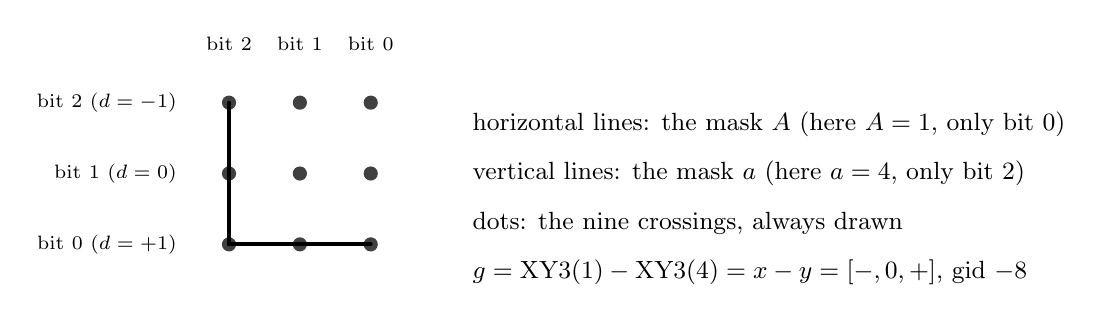
\begin{tikzpicture}[x=9mm,y=9mm,>=stealth]
\foreach \x in {0,1,2}{\foreach \y in {0,1,2}{\fill[black!75] (\x,\y) circle (0.1);}}
\draw[line width=1.4pt,line cap=round] (0,0)--(2,0);
\draw[line width=1.4pt,line cap=round] (0,0)--(0,2);
\node[left] at (-0.6,2) {\scriptsize bit 2 ($d=-1$)};\node[left] at (-0.6,1) {\scriptsize bit 1 ($d=0$)};\node[left] at (-0.6,0) {\scriptsize bit 0 ($d=+1$)};
\node[above] at (0,2.6) {\scriptsize bit 2};\node[above] at (1,2.6) {\scriptsize bit 1};\node[above] at (2,2.6) {\scriptsize bit 0};
\node[right,align=left] at (3.3,1.7) {\small horizontal lines: the mask $A$ (here $A=1$, only bit 0)};
\node[right,align=left] at (3.3,1.0) {\small vertical lines: the mask $a$ (here $a=4$, only bit 2)};
\node[right,align=left] at (3.3,0.3) {\small dots: the nine crossings, always drawn};
\node[right,align=left] at (3.3,-0.4) {\small $g=\mathrm{XY3}(1)-\mathrm{XY3}(4)=x-y=[-,0,+]$, gid $-8$};
\end{tikzpicture}\\[2pt]{\small Figure S17. The hexaogram (hexa-o-gram, ``o'' for orthogonal) of a G3 function, here $(A,a)=(1,4)$: the bits of $A$ are horizontal lines, the bits of $a$ vertical lines.}\end{center}

\textbf{XY3.} Values are those of the mask at the states $(0,1),(0,0),(1,0)$ ($d=-1,0,+1$). The Boolean formulas $x,y,\dots$ agree with the masks on the three states only; at $(1,1)$ they take other values (for example $x\vee y=1$ there, whereas the zon state has the value $0$), which is why the domain is restricted to the three states or $(1,1)$ is sent to the zon state.
\begin{center}\small\renewcommand{\arraystretch}{1.35}\begin{tabular}{rlllccc}\toprule id&mask&trigram&function&$d=-1$&$d=0$&$d=+1$\\\midrule
$0$&\texttt{0b000}&\tri{\yin}{\yin}{\yin} \ Kun&$0$&$0$&$0$&$0$\\
$1$&\texttt{0b001}&\tri{\yin}{\yin}{\yang} \ Zhen&$x$&$0$&$0$&$+$\\
$2$&\texttt{0b010}&\tri{\yin}{\yang}{\yin} \ Kan&$x'y'$&$0$&$+$&$0$\\
$3$&\texttt{0b011}&\tri{\yin}{\yang}{\yang} \ Dui&$y'$&$0$&$+$&$+$\\
$4$&\texttt{0b100}&\tri{\yang}{\yin}{\yin} \ Gen&$y$&$+$&$0$&$0$\\
$5$&\texttt{0b101}&\tri{\yang}{\yin}{\yang} \ Li&$x\vee y$&$+$&$0$&$+$\\
$6$&\texttt{0b110}&\tri{\yang}{\yang}{\yin} \ Xun&$x'$&$+$&$+$&$0$\\
$7$&\texttt{0b111}&\tri{\yang}{\yang}{\yang} \ Qian&$1$&$+$&$+$&$+$\\
\bottomrule\end{tabular}\end{center}

\textbf{G3.} Pairs $(A,a)$ are the XY3 ids of the two masks; $g=[g(-1),g(0),g(+1)]$. The \emph{hexaogram} column draws the two masks superposed, as a $3\times3$ grid of three horizontal and three vertical lines, six lines in all (Figure S17): the three bits of $A$ are the horizontal lines, the three bits of $a$ the vertical lines, and a line is present exactly where its bit is $1$; the nine crossing points are always marked by small dots, so that the position of an absent line can be read. The \emph{bi-trigram} column writes the trigram of $A$ and the trigram of $a$ side by side (top line = bit 2). Both symbols are generated from the pair $(A,a)$ by the same program that builds the table, so symbol, code and function cannot disagree.
\begin{center}\scriptsize\renewcommand{\arraystretch}{1.5}\begin{longtable}{rllccccccp{4.1cm}}\toprule gid&T3 code&$(A,a)$&Hexaogram $(A,a)$&Bi-trigram $(A,a)$&$\mathrm{XY3}(A)-\mathrm{XY3}(a)$&$g$&size&\chai{} term\\\midrule\endhead
$-13$&\texttt{0t222}&(0,7)&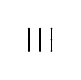
\begin{tikzpicture}[x=0.41em,y=0.40em,baseline=0.25em]\fill[black!75] (0,0) circle (0.04em);\fill[black!75] (0,1) circle (0.04em);\fill[black!75] (0,2) circle (0.04em);\fill[black!75] (1,0) circle (0.04em);\fill[black!75] (1,1) circle (0.04em);\fill[black!75] (1,2) circle (0.04em);\fill[black!75] (2,0) circle (0.04em);\fill[black!75] (2,1) circle (0.04em);\fill[black!75] (2,2) circle (0.04em);\draw[line width=0.6pt,line cap=round] (0,0)--(0,2);\draw[line width=0.6pt,line cap=round] (1,0)--(1,2);\draw[line width=0.6pt,line cap=round] (2,0)--(2,2);\end{tikzpicture}&\tri{\yin}{\yin}{\yin}\ \hspace{0.05em}\tri{\yang}{\yang}{\yang}&$-1$&$[-,-,-]$&3&\texttt{ANT(\allowbreak NOT(\allowbreak DIF(\allowbreak a,\allowbreak a)))}\\
$-12$&\texttt{0t220}&(0,6)&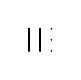
\begin{tikzpicture}[x=0.41em,y=0.40em,baseline=0.25em]\fill[black!75] (0,0) circle (0.04em);\fill[black!75] (0,1) circle (0.04em);\fill[black!75] (0,2) circle (0.04em);\fill[black!75] (1,0) circle (0.04em);\fill[black!75] (1,1) circle (0.04em);\fill[black!75] (1,2) circle (0.04em);\fill[black!75] (2,0) circle (0.04em);\fill[black!75] (2,1) circle (0.04em);\fill[black!75] (2,2) circle (0.04em);\draw[line width=0.6pt,line cap=round] (0,0)--(0,2);\draw[line width=0.6pt,line cap=round] (1,0)--(1,2);\end{tikzpicture}&\tri{\yin}{\yin}{\yin}\ \hspace{0.05em}\tri{\yang}{\yang}{\yin}&$-x'$&$[-,-,0]$&2&\texttt{ANT(\allowbreak NOT(\allowbreak a))}\\
$-11$&\texttt{0t221}&(1,6)&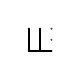
\begin{tikzpicture}[x=0.41em,y=0.40em,baseline=0.25em]\fill[black!75] (0,0) circle (0.04em);\fill[black!75] (0,1) circle (0.04em);\fill[black!75] (0,2) circle (0.04em);\fill[black!75] (1,0) circle (0.04em);\fill[black!75] (1,1) circle (0.04em);\fill[black!75] (1,2) circle (0.04em);\fill[black!75] (2,0) circle (0.04em);\fill[black!75] (2,1) circle (0.04em);\fill[black!75] (2,2) circle (0.04em);\draw[line width=0.6pt,line cap=round] (0,0)--(2,0);\draw[line width=0.6pt,line cap=round] (0,0)--(0,2);\draw[line width=0.6pt,line cap=round] (1,0)--(1,2);\end{tikzpicture}&\tri{\yin}{\yin}{\yang}\ \hspace{0.05em}\tri{\yang}{\yang}{\yin}&$x-x'$&$[-,-,+]$&2&\texttt{DIF(\allowbreak a,\allowbreak NOT(\allowbreak a))}\\
$-10$&\texttt{0t202}&(0,5)&\begin{tikzpicture}[x=0.41em,y=0.40em,baseline=0.25em]\fill[black!75] (0,0) circle (0.04em);\fill[black!75] (0,1) circle (0.04em);\fill[black!75] (0,2) circle (0.04em);\fill[black!75] (1,0) circle (0.04em);\fill[black!75] (1,1) circle (0.04em);\fill[black!75] (1,2) circle (0.04em);\fill[black!75] (2,0) circle (0.04em);\fill[black!75] (2,1) circle (0.04em);\fill[black!75] (2,2) circle (0.04em);\draw[line width=0.6pt,line cap=round] (0,0)--(0,2);\draw[line width=0.6pt,line cap=round] (2,0)--(2,2);\end{tikzpicture}&\tri{\yin}{\yin}{\yin}\ \hspace{0.05em}\tri{\yang}{\yin}{\yang}&$-(x\vee y)$&$[-,0,-]$&2&\texttt{AND(\allowbreak ANT(\allowbreak a),\allowbreak a)}\\
$-9$&\texttt{0t200}&(0,4)&\begin{tikzpicture}[x=0.41em,y=0.40em,baseline=0.25em]\fill[black!75] (0,0) circle (0.04em);\fill[black!75] (0,1) circle (0.04em);\fill[black!75] (0,2) circle (0.04em);\fill[black!75] (1,0) circle (0.04em);\fill[black!75] (1,1) circle (0.04em);\fill[black!75] (1,2) circle (0.04em);\fill[black!75] (2,0) circle (0.04em);\fill[black!75] (2,1) circle (0.04em);\fill[black!75] (2,2) circle (0.04em);\draw[line width=0.6pt,line cap=round] (0,0)--(0,2);\end{tikzpicture}&\tri{\yin}{\yin}{\yin}\ \hspace{0.05em}\tri{\yang}{\yin}{\yin}&$-y$&$[-,0,0]$&2&\texttt{AND(\allowbreak NOT(\allowbreak a),\allowbreak a)}\\
$-8$&\texttt{0t201}&(1,4)&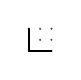
\begin{tikzpicture}[x=0.41em,y=0.40em,baseline=0.25em]\fill[black!75] (0,0) circle (0.04em);\fill[black!75] (0,1) circle (0.04em);\fill[black!75] (0,2) circle (0.04em);\fill[black!75] (1,0) circle (0.04em);\fill[black!75] (1,1) circle (0.04em);\fill[black!75] (1,2) circle (0.04em);\fill[black!75] (2,0) circle (0.04em);\fill[black!75] (2,1) circle (0.04em);\fill[black!75] (2,2) circle (0.04em);\draw[line width=0.6pt,line cap=round] (0,0)--(2,0);\draw[line width=0.6pt,line cap=round] (0,0)--(0,2);\end{tikzpicture}&\tri{\yin}{\yin}{\yang}\ \hspace{0.05em}\tri{\yang}{\yin}{\yin}&$x-y$&$[-,0,+]$&0&\texttt{a}\\
$-7$&\texttt{0t212}&(2,5)&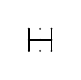
\begin{tikzpicture}[x=0.41em,y=0.40em,baseline=0.25em]\fill[black!75] (0,0) circle (0.04em);\fill[black!75] (0,1) circle (0.04em);\fill[black!75] (0,2) circle (0.04em);\fill[black!75] (1,0) circle (0.04em);\fill[black!75] (1,1) circle (0.04em);\fill[black!75] (1,2) circle (0.04em);\fill[black!75] (2,0) circle (0.04em);\fill[black!75] (2,1) circle (0.04em);\fill[black!75] (2,2) circle (0.04em);\draw[line width=0.6pt,line cap=round] (0,1)--(2,1);\draw[line width=0.6pt,line cap=round] (0,0)--(0,2);\draw[line width=0.6pt,line cap=round] (2,0)--(2,2);\end{tikzpicture}&\tri{\yin}{\yang}{\yin}\ \hspace{0.05em}\tri{\yang}{\yin}{\yang}&$x'y'-(x\vee y)$&$[-,+,-]$&4&\texttt{DIF(\allowbreak NOT(\allowbreak AND(\allowbreak a,\allowbreak a)),\allowbreak AND(\allowbreak a,\allowbreak a))}\\
$-6$&\texttt{0t210}&(2,4)&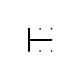
\begin{tikzpicture}[x=0.41em,y=0.40em,baseline=0.25em]\fill[black!75] (0,0) circle (0.04em);\fill[black!75] (0,1) circle (0.04em);\fill[black!75] (0,2) circle (0.04em);\fill[black!75] (1,0) circle (0.04em);\fill[black!75] (1,1) circle (0.04em);\fill[black!75] (1,2) circle (0.04em);\fill[black!75] (2,0) circle (0.04em);\fill[black!75] (2,1) circle (0.04em);\fill[black!75] (2,2) circle (0.04em);\draw[line width=0.6pt,line cap=round] (0,1)--(2,1);\draw[line width=0.6pt,line cap=round] (0,0)--(0,2);\end{tikzpicture}&\tri{\yin}{\yang}{\yin}\ \hspace{0.05em}\tri{\yang}{\yin}{\yin}&$x'y'-y$&$[-,+,0]$&4&\texttt{DIF(\allowbreak NOT(\allowbreak ANT(\allowbreak a)),\allowbreak AND(\allowbreak a,\allowbreak a))}\\
$-5$&\texttt{0t211}&(3,4)&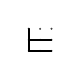
\begin{tikzpicture}[x=0.41em,y=0.40em,baseline=0.25em]\fill[black!75] (0,0) circle (0.04em);\fill[black!75] (0,1) circle (0.04em);\fill[black!75] (0,2) circle (0.04em);\fill[black!75] (1,0) circle (0.04em);\fill[black!75] (1,1) circle (0.04em);\fill[black!75] (1,2) circle (0.04em);\fill[black!75] (2,0) circle (0.04em);\fill[black!75] (2,1) circle (0.04em);\fill[black!75] (2,2) circle (0.04em);\draw[line width=0.6pt,line cap=round] (0,1)--(2,1);\draw[line width=0.6pt,line cap=round] (0,0)--(2,0);\draw[line width=0.6pt,line cap=round] (0,0)--(0,2);\end{tikzpicture}&\tri{\yin}{\yang}{\yang}\ \hspace{0.05em}\tri{\yang}{\yin}{\yin}&$y'-y$&$[-,+,+]$&3&\texttt{SYN(\allowbreak NOT(\allowbreak AND(\allowbreak a,\allowbreak a)),\allowbreak a)}\\
$-4$&\texttt{0t022}&(0,3)&\begin{tikzpicture}[x=0.41em,y=0.40em,baseline=0.25em]\fill[black!75] (0,0) circle (0.04em);\fill[black!75] (0,1) circle (0.04em);\fill[black!75] (0,2) circle (0.04em);\fill[black!75] (1,0) circle (0.04em);\fill[black!75] (1,1) circle (0.04em);\fill[black!75] (1,2) circle (0.04em);\fill[black!75] (2,0) circle (0.04em);\fill[black!75] (2,1) circle (0.04em);\fill[black!75] (2,2) circle (0.04em);\draw[line width=0.6pt,line cap=round] (1,0)--(1,2);\draw[line width=0.6pt,line cap=round] (2,0)--(2,2);\end{tikzpicture}&\tri{\yin}{\yin}{\yin}\ \hspace{0.05em}\tri{\yin}{\yang}{\yang}&$-y'$&$[0,-,-]$&3&\texttt{ANT(\allowbreak NOT(\allowbreak ANT(\allowbreak a)))}\\
$-3$&\texttt{0t020}&(0,2)&\begin{tikzpicture}[x=0.41em,y=0.40em,baseline=0.25em]\fill[black!75] (0,0) circle (0.04em);\fill[black!75] (0,1) circle (0.04em);\fill[black!75] (0,2) circle (0.04em);\fill[black!75] (1,0) circle (0.04em);\fill[black!75] (1,1) circle (0.04em);\fill[black!75] (1,2) circle (0.04em);\fill[black!75] (2,0) circle (0.04em);\fill[black!75] (2,1) circle (0.04em);\fill[black!75] (2,2) circle (0.04em);\draw[line width=0.6pt,line cap=round] (1,0)--(1,2);\end{tikzpicture}&\tri{\yin}{\yin}{\yin}\ \hspace{0.05em}\tri{\yin}{\yang}{\yin}&$-x'y'$&$[0,-,0]$&3&\texttt{ANT(\allowbreak NOT(\allowbreak AND(\allowbreak a,\allowbreak a)))}\\
$-2$&\texttt{0t021}&(1,2)&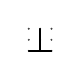
\begin{tikzpicture}[x=0.41em,y=0.40em,baseline=0.25em]\fill[black!75] (0,0) circle (0.04em);\fill[black!75] (0,1) circle (0.04em);\fill[black!75] (0,2) circle (0.04em);\fill[black!75] (1,0) circle (0.04em);\fill[black!75] (1,1) circle (0.04em);\fill[black!75] (1,2) circle (0.04em);\fill[black!75] (2,0) circle (0.04em);\fill[black!75] (2,1) circle (0.04em);\fill[black!75] (2,2) circle (0.04em);\draw[line width=0.6pt,line cap=round] (0,0)--(2,0);\draw[line width=0.6pt,line cap=round] (1,0)--(1,2);\end{tikzpicture}&\tri{\yin}{\yin}{\yang}\ \hspace{0.05em}\tri{\yin}{\yang}{\yin}&$x-x'y'$&$[0,-,+]$&3&\texttt{DIF(\allowbreak AND(\allowbreak a,\allowbreak a),\allowbreak NOT(\allowbreak a))}\\
$-1$&\texttt{0t002}&(0,1)&\begin{tikzpicture}[x=0.41em,y=0.40em,baseline=0.25em]\fill[black!75] (0,0) circle (0.04em);\fill[black!75] (0,1) circle (0.04em);\fill[black!75] (0,2) circle (0.04em);\fill[black!75] (1,0) circle (0.04em);\fill[black!75] (1,1) circle (0.04em);\fill[black!75] (1,2) circle (0.04em);\fill[black!75] (2,0) circle (0.04em);\fill[black!75] (2,1) circle (0.04em);\fill[black!75] (2,2) circle (0.04em);\draw[line width=0.6pt,line cap=round] (2,0)--(2,2);\end{tikzpicture}&\tri{\yin}{\yin}{\yin}\ \hspace{0.05em}\tri{\yin}{\yin}{\yang}&$-x$&$[0,0,-]$&3&\texttt{ANT(\allowbreak NOT(\allowbreak NOT(\allowbreak a)))}\\
$0$&\texttt{0t000}&(0,0)&\begin{tikzpicture}[x=0.41em,y=0.40em,baseline=0.25em]\fill[black!75] (0,0) circle (0.04em);\fill[black!75] (0,1) circle (0.04em);\fill[black!75] (0,2) circle (0.04em);\fill[black!75] (1,0) circle (0.04em);\fill[black!75] (1,1) circle (0.04em);\fill[black!75] (1,2) circle (0.04em);\fill[black!75] (2,0) circle (0.04em);\fill[black!75] (2,1) circle (0.04em);\fill[black!75] (2,2) circle (0.04em);\end{tikzpicture}&\tri{\yin}{\yin}{\yin}\ \hspace{0.05em}\tri{\yin}{\yin}{\yin}&$0$&$[0,0,0]$&1&\texttt{DIF(\allowbreak a,\allowbreak a)}\\
$1$&\texttt{0t001}&(1,0)&\begin{tikzpicture}[x=0.41em,y=0.40em,baseline=0.25em]\fill[black!75] (0,0) circle (0.04em);\fill[black!75] (0,1) circle (0.04em);\fill[black!75] (0,2) circle (0.04em);\fill[black!75] (1,0) circle (0.04em);\fill[black!75] (1,1) circle (0.04em);\fill[black!75] (1,2) circle (0.04em);\fill[black!75] (2,0) circle (0.04em);\fill[black!75] (2,1) circle (0.04em);\fill[black!75] (2,2) circle (0.04em);\draw[line width=0.6pt,line cap=round] (0,0)--(2,0);\end{tikzpicture}&\tri{\yin}{\yin}{\yang}\ \hspace{0.05em}\tri{\yin}{\yin}{\yin}&$x$&$[0,0,+]$&2&\texttt{NOT(\allowbreak NOT(\allowbreak a))}\\
$2$&\texttt{0t012}&(2,1)&\begin{tikzpicture}[x=0.41em,y=0.40em,baseline=0.25em]\fill[black!75] (0,0) circle (0.04em);\fill[black!75] (0,1) circle (0.04em);\fill[black!75] (0,2) circle (0.04em);\fill[black!75] (1,0) circle (0.04em);\fill[black!75] (1,1) circle (0.04em);\fill[black!75] (1,2) circle (0.04em);\fill[black!75] (2,0) circle (0.04em);\fill[black!75] (2,1) circle (0.04em);\fill[black!75] (2,2) circle (0.04em);\draw[line width=0.6pt,line cap=round] (0,1)--(2,1);\draw[line width=0.6pt,line cap=round] (2,0)--(2,2);\end{tikzpicture}&\tri{\yin}{\yang}{\yin}\ \hspace{0.05em}\tri{\yin}{\yin}{\yang}&$x'y'-x$&$[0,+,-]$&3&\texttt{DIF(\allowbreak NOT(\allowbreak a),\allowbreak AND(\allowbreak a,\allowbreak a))}\\
$3$&\texttt{0t010}&(2,0)&\begin{tikzpicture}[x=0.41em,y=0.40em,baseline=0.25em]\fill[black!75] (0,0) circle (0.04em);\fill[black!75] (0,1) circle (0.04em);\fill[black!75] (0,2) circle (0.04em);\fill[black!75] (1,0) circle (0.04em);\fill[black!75] (1,1) circle (0.04em);\fill[black!75] (1,2) circle (0.04em);\fill[black!75] (2,0) circle (0.04em);\fill[black!75] (2,1) circle (0.04em);\fill[black!75] (2,2) circle (0.04em);\draw[line width=0.6pt,line cap=round] (0,1)--(2,1);\end{tikzpicture}&\tri{\yin}{\yang}{\yin}\ \hspace{0.05em}\tri{\yin}{\yin}{\yin}&$x'y'$&$[0,+,0]$&2&\texttt{NOT(\allowbreak AND(\allowbreak a,\allowbreak a))}\\
$4$&\texttt{0t011}&(3,0)&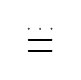
\begin{tikzpicture}[x=0.41em,y=0.40em,baseline=0.25em]\fill[black!75] (0,0) circle (0.04em);\fill[black!75] (0,1) circle (0.04em);\fill[black!75] (0,2) circle (0.04em);\fill[black!75] (1,0) circle (0.04em);\fill[black!75] (1,1) circle (0.04em);\fill[black!75] (1,2) circle (0.04em);\fill[black!75] (2,0) circle (0.04em);\fill[black!75] (2,1) circle (0.04em);\fill[black!75] (2,2) circle (0.04em);\draw[line width=0.6pt,line cap=round] (0,1)--(2,1);\draw[line width=0.6pt,line cap=round] (0,0)--(2,0);\end{tikzpicture}&\tri{\yin}{\yang}{\yang}\ \hspace{0.05em}\tri{\yin}{\yin}{\yin}&$y'$&$[0,+,+]$&2&\texttt{NOT(\allowbreak ANT(\allowbreak a))}\\
$5$&\texttt{0t122}&(4,3)&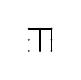
\begin{tikzpicture}[x=0.41em,y=0.40em,baseline=0.25em]\fill[black!75] (0,0) circle (0.04em);\fill[black!75] (0,1) circle (0.04em);\fill[black!75] (0,2) circle (0.04em);\fill[black!75] (1,0) circle (0.04em);\fill[black!75] (1,1) circle (0.04em);\fill[black!75] (1,2) circle (0.04em);\fill[black!75] (2,0) circle (0.04em);\fill[black!75] (2,1) circle (0.04em);\fill[black!75] (2,2) circle (0.04em);\draw[line width=0.6pt,line cap=round] (0,2)--(2,2);\draw[line width=0.6pt,line cap=round] (1,0)--(1,2);\draw[line width=0.6pt,line cap=round] (2,0)--(2,2);\end{tikzpicture}&\tri{\yang}{\yin}{\yin}\ \hspace{0.05em}\tri{\yin}{\yang}{\yang}&$y-y'$&$[+,-,-]$&4&\texttt{ANT(\allowbreak SYN(\allowbreak NOT(\allowbreak AND(\allowbreak a,\allowbreak a)),\allowbreak a))}\\
$6$&\texttt{0t120}&(4,2)&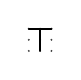
\begin{tikzpicture}[x=0.41em,y=0.40em,baseline=0.25em]\fill[black!75] (0,0) circle (0.04em);\fill[black!75] (0,1) circle (0.04em);\fill[black!75] (0,2) circle (0.04em);\fill[black!75] (1,0) circle (0.04em);\fill[black!75] (1,1) circle (0.04em);\fill[black!75] (1,2) circle (0.04em);\fill[black!75] (2,0) circle (0.04em);\fill[black!75] (2,1) circle (0.04em);\fill[black!75] (2,2) circle (0.04em);\draw[line width=0.6pt,line cap=round] (0,2)--(2,2);\draw[line width=0.6pt,line cap=round] (1,0)--(1,2);\end{tikzpicture}&\tri{\yang}{\yin}{\yin}\ \hspace{0.05em}\tri{\yin}{\yang}{\yin}&$y-x'y'$&$[+,-,0]$&4&\texttt{DIF(\allowbreak AND(\allowbreak a,\allowbreak a),\allowbreak NOT(\allowbreak ANT(\allowbreak a)))}\\
$7$&\texttt{0t121}&(5,2)&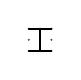
\begin{tikzpicture}[x=0.41em,y=0.40em,baseline=0.25em]\fill[black!75] (0,0) circle (0.04em);\fill[black!75] (0,1) circle (0.04em);\fill[black!75] (0,2) circle (0.04em);\fill[black!75] (1,0) circle (0.04em);\fill[black!75] (1,1) circle (0.04em);\fill[black!75] (1,2) circle (0.04em);\fill[black!75] (2,0) circle (0.04em);\fill[black!75] (2,1) circle (0.04em);\fill[black!75] (2,2) circle (0.04em);\draw[line width=0.6pt,line cap=round] (0,2)--(2,2);\draw[line width=0.6pt,line cap=round] (0,0)--(2,0);\draw[line width=0.6pt,line cap=round] (1,0)--(1,2);\end{tikzpicture}&\tri{\yang}{\yin}{\yang}\ \hspace{0.05em}\tri{\yin}{\yang}{\yin}&$x\vee y-x'y'$&$[+,-,+]$&4&\texttt{DIF(\allowbreak AND(\allowbreak a,\allowbreak a),\allowbreak NOT(\allowbreak AND(\allowbreak a,\allowbreak a)))}\\
$8$&\texttt{0t102}&(4,1)&\begin{tikzpicture}[x=0.41em,y=0.40em,baseline=0.25em]\fill[black!75] (0,0) circle (0.04em);\fill[black!75] (0,1) circle (0.04em);\fill[black!75] (0,2) circle (0.04em);\fill[black!75] (1,0) circle (0.04em);\fill[black!75] (1,1) circle (0.04em);\fill[black!75] (1,2) circle (0.04em);\fill[black!75] (2,0) circle (0.04em);\fill[black!75] (2,1) circle (0.04em);\fill[black!75] (2,2) circle (0.04em);\draw[line width=0.6pt,line cap=round] (0,2)--(2,2);\draw[line width=0.6pt,line cap=round] (2,0)--(2,2);\end{tikzpicture}&\tri{\yang}{\yin}{\yin}\ \hspace{0.05em}\tri{\yin}{\yin}{\yang}&$y-x$&$[+,0,-]$&1&\texttt{ANT(\allowbreak a)}\\
$9$&\texttt{0t100}&(4,0)&\begin{tikzpicture}[x=0.41em,y=0.40em,baseline=0.25em]\fill[black!75] (0,0) circle (0.04em);\fill[black!75] (0,1) circle (0.04em);\fill[black!75] (0,2) circle (0.04em);\fill[black!75] (1,0) circle (0.04em);\fill[black!75] (1,1) circle (0.04em);\fill[black!75] (1,2) circle (0.04em);\fill[black!75] (2,0) circle (0.04em);\fill[black!75] (2,1) circle (0.04em);\fill[black!75] (2,2) circle (0.04em);\draw[line width=0.6pt,line cap=round] (0,2)--(2,2);\end{tikzpicture}&\tri{\yang}{\yin}{\yin}\ \hspace{0.05em}\tri{\yin}{\yin}{\yin}&$y$&$[+,0,0]$&2&\texttt{DIF(\allowbreak AND(\allowbreak a,\allowbreak a),\allowbreak a)}\\
$10$&\texttt{0t101}&(5,0)&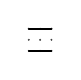
\begin{tikzpicture}[x=0.41em,y=0.40em,baseline=0.25em]\fill[black!75] (0,0) circle (0.04em);\fill[black!75] (0,1) circle (0.04em);\fill[black!75] (0,2) circle (0.04em);\fill[black!75] (1,0) circle (0.04em);\fill[black!75] (1,1) circle (0.04em);\fill[black!75] (1,2) circle (0.04em);\fill[black!75] (2,0) circle (0.04em);\fill[black!75] (2,1) circle (0.04em);\fill[black!75] (2,2) circle (0.04em);\draw[line width=0.6pt,line cap=round] (0,2)--(2,2);\draw[line width=0.6pt,line cap=round] (0,0)--(2,0);\end{tikzpicture}&\tri{\yang}{\yin}{\yang}\ \hspace{0.05em}\tri{\yin}{\yin}{\yin}&$x\vee y$&$[+,0,+]$&1&\texttt{AND(\allowbreak a,\allowbreak a)}\\
$11$&\texttt{0t112}&(6,1)&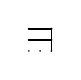
\begin{tikzpicture}[x=0.41em,y=0.40em,baseline=0.25em]\fill[black!75] (0,0) circle (0.04em);\fill[black!75] (0,1) circle (0.04em);\fill[black!75] (0,2) circle (0.04em);\fill[black!75] (1,0) circle (0.04em);\fill[black!75] (1,1) circle (0.04em);\fill[black!75] (1,2) circle (0.04em);\fill[black!75] (2,0) circle (0.04em);\fill[black!75] (2,1) circle (0.04em);\fill[black!75] (2,2) circle (0.04em);\draw[line width=0.6pt,line cap=round] (0,2)--(2,2);\draw[line width=0.6pt,line cap=round] (0,1)--(2,1);\draw[line width=0.6pt,line cap=round] (2,0)--(2,2);\end{tikzpicture}&\tri{\yang}{\yang}{\yin}\ \hspace{0.05em}\tri{\yin}{\yin}{\yang}&$x'-x$&$[+,+,-]$&2&\texttt{DIF(\allowbreak NOT(\allowbreak a),\allowbreak a)}\\
$12$&\texttt{0t110}&(6,0)&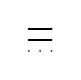
\begin{tikzpicture}[x=0.41em,y=0.40em,baseline=0.25em]\fill[black!75] (0,0) circle (0.04em);\fill[black!75] (0,1) circle (0.04em);\fill[black!75] (0,2) circle (0.04em);\fill[black!75] (1,0) circle (0.04em);\fill[black!75] (1,1) circle (0.04em);\fill[black!75] (1,2) circle (0.04em);\fill[black!75] (2,0) circle (0.04em);\fill[black!75] (2,1) circle (0.04em);\fill[black!75] (2,2) circle (0.04em);\draw[line width=0.6pt,line cap=round] (0,2)--(2,2);\draw[line width=0.6pt,line cap=round] (0,1)--(2,1);\end{tikzpicture}&\tri{\yang}{\yang}{\yin}\ \hspace{0.05em}\tri{\yin}{\yin}{\yin}&$x'$&$[+,+,0]$&1&\texttt{NOT(\allowbreak a)}\\
$13$&\texttt{0t111}&(7,0)&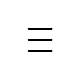
\begin{tikzpicture}[x=0.41em,y=0.40em,baseline=0.25em]\fill[black!75] (0,0) circle (0.04em);\fill[black!75] (0,1) circle (0.04em);\fill[black!75] (0,2) circle (0.04em);\fill[black!75] (1,0) circle (0.04em);\fill[black!75] (1,1) circle (0.04em);\fill[black!75] (1,2) circle (0.04em);\fill[black!75] (2,0) circle (0.04em);\fill[black!75] (2,1) circle (0.04em);\fill[black!75] (2,2) circle (0.04em);\draw[line width=0.6pt,line cap=round] (0,2)--(2,2);\draw[line width=0.6pt,line cap=round] (0,1)--(2,1);\draw[line width=0.6pt,line cap=round] (0,0)--(2,0);\end{tikzpicture}&\tri{\yang}{\yang}{\yang}\ \hspace{0.05em}\tri{\yin}{\yin}{\yin}&$1$&$[+,+,+]$&2&\texttt{NOT(\allowbreak DIF(\allowbreak a,\allowbreak a))}\\
\bottomrule\end{longtable}\end{center}
\textbf{Selectors.} On the three states the functions $x$, $x'y'$, $y$ (the masks $1$, $2$, $4$) are one-hot. At $(1,1)$ both $x$ and $y$ equal $1$ and $x'y'=0$, so a sum of the three products with these Boolean selectors would add two branches there; the total selector of the paper (S8) sends $(1,1)$ to the zon branch instead. The C9 layer is the three-branch selection of S9.

\section*{S18. Checks added for this version}
The standard-library program \texttt{chai\_verify\_v1\_increments.py} (123 checks, all passed; results in \texttt{chaiv1\_increments\_results.json}) evaluates, from the primitive definitions, the statements that are new in this version of the paper, and the explicit constructions of its proofs on \emph{every} binary function of the classes, not on samples:
\begin{itemize}\setlength\itemsep{0pt}
\item Section II: the three sections $\NOT=[+,+,0]$, $\ANT=[+,0,-]$, $\DIF(-1,\cdot)=[0,-,-]=-\NOT(-\cdot)$; that only the section at $0$ is an involution; $\NOT\circ\NOT=[0,0,+]$; the least $\DIF$-closed set containing $\{0,1\}$ is $\{-1,0,+1\}$ (iteration); $\DIF(-1,+1)=-1\ne-2$.
\item The printed Tables I, II and III against the definitions: all five binary tables and the three unary rows cell by cell; the five columns of Table II for the seven primitives; the numbers $3,81,12,3888,9,6561,27,19\,683$ of Table III.
\item Lemma 2 and Theorems 3--5: $\delta_p$ for the eight $p\ne0$; all $6561$ functions of $\Z_2$ from the five operations; all $19\,683$ binary functions as $\SYN\big(F',\AND(e_0,F(0))\big)$ (Theorem 3(c)); all $81$ odd binary functions from $\DIF$ alone with the terms $k_c$ and $s_p$; all $3888$ functions of $\mathcal B_2$ and $300$ random functions of $\mathcal B_3$ from $\SYN,\OR,\XOR,\AND,\NOT$.
\item Theorem 6: the criterion ``$\NOT\in\Sigma$ and ($\DIF\in\Sigma$ or $\{\SYN,\ANT\}\subseteq\Sigma$)'' agrees with all $127$ rows of \texttt{classification\_127.csv}, and $40$ rows are complete; the relation $\rho$ is preserved by $\ANT,\OR,\XOR,\AND,\NOT$ and not by $\SYN$ or $\DIF$; the witnesses of the necessity proof, $\DIF(0,+1)=-1\notin B$ and $(\DIF(+1,0),\DIF(0,+1))=(+1,-1)\notin\rho$; the five closures with constants of Table~IV of the paper against the shipped \texttt{results\_consts\_*.json} (size $19\,683$ and last height).
\item Sections III and VI: parity lemma and polarization at the nine pairs, the failure at $(2,1)$ on $\{-2,\dots,2\}$, $\Phi$ an involution with one fixed point, the congruence of the fold ($\AND$ and $\ANT$ only), the clockwise rotation of the five tables, $\MAX,\MIN$ as terms, the associativity failures $4,16,8,8$, the Shannon/Post expansion on $500$ random binary functions, the T9ID words of $\SYN$ and $\DIF$, the order-$8$ group and the Burnside count $2862$.
\end{itemize}
The large closures (the $6561$, $3888$ and $19\,683$ binary functions as closures of the projections) and the closures with nullary constants are not recomputed here; they are those of the earlier verified runs (\texttt{results.json}, \texttt{results\_consts\_*.json}) for the same seven operations.

\section*{S19. Structure of \chai{}: the diagram of the earlier version}
Figure S19 is the structure diagram of the earlier version of the paper, kept here because it shows the relations among the seven operations at a glance. Each arrow is a statement proved in the paper. Arrows from $(a,b)$ to $\SYN$ and $\DIF$: the pair $\Phi=(\SYN,\DIF)$ is an involution (Theorem~2). Vertical arrows labelled $\MAG$: folding the sum or the difference to its magnitude gives $\OR=\MAG\circ\SYN$ and $\XOR=\MAG\circ\DIF$. Arrows from $\OR$ and $\XOR$ to $\AND$: the polarization $\AND=\DIF(\OR,\XOR)$ (Theorem~1). Dashed double arrows: replacing the second argument $b$ by $\ANT(b)$ exchanges $\SYN\leftrightarrow\DIF$ and $\OR\leftrightarrow\XOR$, since $\SYN(a,b)=\DIF(a,\ANT(b))$ and $\OR(a,\ANT(b))=\XOR(a,b)$. The dotted rectangle is the zero-fixing clone $\Z$ ($f(0,\dots,0)=0$): the five binary operations stay inside it (Theorem~3a,b), while $\NOT$ is zero-breaking and, together with the five, gives all of $\Fone$ and $\Ftwo$ (Theorem~3c).
\begin{center}
\resizebox{0.8\textwidth}{!}{%
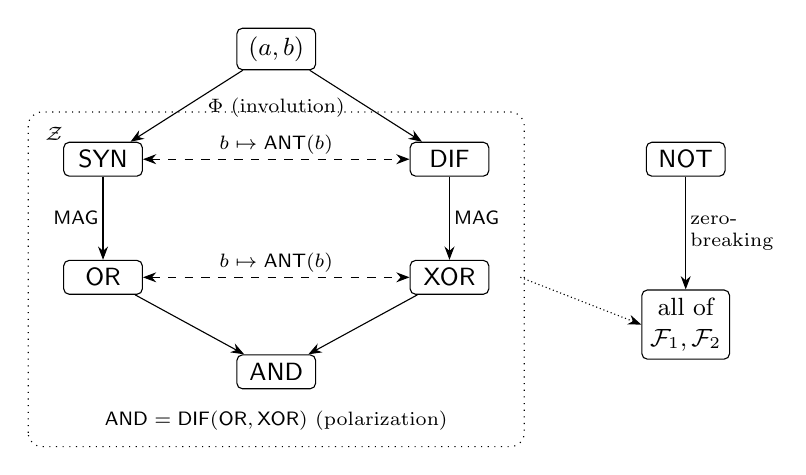
\begin{tikzpicture}[>=Stealth,font=\small,
box/.style={draw,rounded corners=2pt,inner sep=3pt,minimum width=1.0cm},
lab/.style={font=\scriptsize,inner sep=1.5pt}]
\node[box] (ab) at (2.2,4.1) {$(a,b)$};
\node[box] (syn) at (0,2.7) {$\SYN$};
\node[box] (dif) at (4.4,2.7) {$\DIF$};
\node[box] (or) at (0,1.2) {$\OR$};
\node[box] (xor) at (4.4,1.2) {$\XOR$};
\node[box] (and) at (2.2,0) {$\AND$};
\draw[->] (ab)--(syn); \draw[->] (ab)--(dif);
\node[lab] at (2.2,3.35) {$\Phi$ (involution)};
\draw[->] (syn)--node[lab,left]{$\MAG$}(or);
\draw[->] (dif)--node[lab,right]{$\MAG$}(xor);
\draw[->] (or)--(and); \draw[->] (xor)--(and);
\node[lab,align=center] at (2.2,-0.62) {$\AND=\DIF(\OR,\XOR)$ (polarization)};
\draw[<->,dashed] (syn)--node[lab,above]{$b\mapsto\ANT(b)$}(dif);
\draw[<->,dashed] (or)--node[lab,above]{$b\mapsto\ANT(b)$}(xor);
\draw[dotted,rounded corners=5pt] (-0.95,-0.95) rectangle (5.35,3.3);
\node[lab] at (-0.62,3.02) {$\Z$};
\node[box] (not) at (7.4,2.7) {$\NOT$};
\node[box,align=center] (all) at (7.4,0.6) {all of\\$\Fone,\Ftwo$};
\draw[->] (not)--node[lab,right,align=left]{zero-\\breaking}(all);
\draw[->,densely dotted] (5.3,1.2)--(all.west);
\end{tikzpicture}}\\[2pt]
{\small Figure S19. Structure of \chai{}. The five binary operations stay inside the zero-fixing clone $\Z$ (dotted; $f(0,\dots,0)=0$), and $\NOT$ leaves it. Dashed arrows: negation of the second argument.}
\end{center}

\end{document}
